\chapter{Design Sensitivity Analysis}\label{ch:sensitivityAnalysis}
In this chapter, the concept of discrete and continuum sensitivity formulation is discussed, and the general approach for deriving the sensitivity equations is presented. Then, the difference between the local and total formulation of the sensitivity response is discussed and finally, the independence of continuum sensitivity analysis to discretization method is proven. This enables us to reuse the solver of governing equations to calculate the sensitivity response. Discrete sensitivity formulation is not capable of using the same solver for both that solution of governing equation and sensitivity analysis. The two sensitivity analysis techniques are applied to a heat transfer benchmark problem where the sensitivity of response to the shape of the domain is calculated. This problem is also used in the next chapter for implementation of different immersed boundary methods.

% ======================================================================================
\section{General Formulation}
The general shape for the computational domain is defined in Figure \ref{fig:C2_continuumDomain}. The response variable on this domain can represent a fluid, i.e. pressure or velocity, or a solid, i.e. displacements. Nevertheless, in any of these cases, the response is calculated by solving a governing equation subjected to boundary conditions. 

\begin{figure}
    \centering
    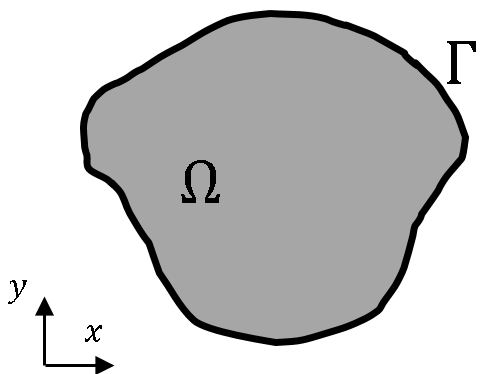
\includegraphics[width=4.00cm]{Chapter_2/figure/general_domain.png}
    \caption{General computational domain $\Omega$ with boundary $\Gamma$.}
    \label{fig:C2_continuumDomain}
\end{figure}

In this research, the governing equation and the boundary conditions are represented in the functional form as shown in Equation \eqref{eq:C2_governingEquationAndBC}.

\begin{subequations}\label{eq:C2_governingEquationAndBC}
\begin{equation}\label{eq:C2_generalGoverningEquation}
    \mathbf{A}(\mathbf{u}, t; \mathbf{b}) = \mathbf{f}(\mathbf{x}, t; \mathbf{b})
    \quad \text{on} \quad \Omega
\end{equation}
\begin{equation}\label{eq:C2_generalBoundaryCondition}
    \mathbf{B}(\mathbf{u}, t; \mathbf{b}) = \mathbf{g}(\mathbf{x}, t; \mathbf{b})    
    \quad \text{on} \quad \Gamma
\end{equation}
\end{subequations}

where $\mathbf{A}$ is the governing equation, such as Navier-Stokes equations for the fluid or elastic equations for the solid domain, and $\mathbf{B}$ is the boundary condition. $\mathbf{u}$ is the response variable such as displacement or pressure. $t$ is time, $\mathbf{b}$ is the design variable such as shape or size, and $\mathbf{x}$ is the spatial coordinate. $\mathbf{f}$ and $\mathbf{g}$ are the values of the governing equation and boundary conditions. It should be noted that in this formulation, the functions $\mathbf{A}$ and $\mathbf{B}$ are only implicitly dependent on the design variable $\mathbf{b}$. This is important when deriving the sensitivity equations later in this chapter. This implicit dependence is represented by using the semicolon symbol in the definition of $\mathbf{A}$ and $\mathbf{B}$.

For the general case of problem formulation, the total sensitivity of response variable, $\mathbf{u}$, with respect to the $i$-th design variable, $b_i$, is written as:

\begin{equation}\label{eq:C2_totalSensitivityDef}
    \frac{D \mathbf{u}}{D b_i} = 
    \underbrace{\frac{\partial \mathbf{u}}{\partial b_i}}_\text{local derivative} + 
    \underbrace{\frac{\partial \mathbf{u}}{\partial \mathbf{x}} \cdot
    \frac{\partial \mathbf{x}}{\partial b_i}}_\text{convective term}
\end{equation}

The total derivative is known as the material derivative in continuum mechanics \cite{mase2009continuum}. This total sensitivity defines the change of response variable, $\mathbf{u}$, to design variable and space dependent changes. The material derivative consists of the local derivative, $\partial \mathbf{u}/\partial b_i$, plus the convective term, $\partial \mathbf{u}/\partial \mathbf{x} \cdot \partial \mathbf{x}/\partial b_i$. The local derivative is the measure of change in the response variable due to change in the design parameter. Whereas, the convective term accounts for the movement of points in space due to change in the design variable. This is especially applicable to shape sensitivity analysis where the change in design variable will cause the material points to move \cite{cross2014local}.

The convective term consists of two separate gradients: i) $\partial \mathbf{u} / \partial \mathbf{x}$ which represents the spatial gradient of the response variable, and ii) $\partial \mathbf{x} / \partial b_i$ that defines the sensitivity of the location of computational nodes with respect to changes in the design variable. The response gradient, $\partial u/\partial x$, is calculated from the analysis results using finite difference approach or derivative of shape functions in FEA formulation. The calculation of domain sensitivity, $\partial \mathbf{x} / \partial b_i$, requires more attention.

A standard approach for calculating the domain sensitivity is to use the techniques used to deform the body-conformal mesh in CFD/FEA simulations. These methods are commonly based on representing the computational grid as a system of springs that connected to each other at the nodes. This system is modeled and solved using structural analysis techniques, where the sensitivities can be easily implemented. This is effectively a shape sensitivity analysis for the structural problem \cite{haftka1986structural}. This step is removed from the analysis if the computational domain is not affected by the design variable since $\partial x/\partial b$ is equal to zero \cite{gobal2014continuum}. This is one of the reasons to use the immersed boundary calculation since it reduces the cost of the simulation. This is discussed in more details in Chapter \ref{ch:immersedBoundary}.

% ======================================================================================
\section{Benchmark Cases}
To compare the discrete and continuum sensitivity analysis formulations, two problems from different disciplines are selected. As a simplified representation for the fluid/thermal systems, the one-dimensional heat transfer analysis in a beam is selected. This problem is used by different researchers for investigating sensitivity analysis for nonlinear systems \cite{dowding2001sensitivity}, thermal design, and monitoring \cite{szopa2005second, sorli2004computational}. The special interest in this problem is due to availability of analytical solution since this can be used to verify the numerical results of the sensitivity analysis. For the solid mechanics problem, a finite element model of an axial bar with distributed load is selected \cite{szabo1991finite}. This problem is used by different researchers as a demonstration case for sensitivity analysis \cite{cross2014local, wickert2009least}. These benchmark cases are explained in more details in the following sections.

% -.-.-.-.-.-.-.-.-.-.-.-.-.-.-.-.-.-.-.-.-.-.-.-.-.-.-.-.-.-.-.-.-.-.-.-.-.-.-.-.-.-.-.
\subsection{Heat transfer benchmark case}
The temperature in the one-dimensional domain is governed by the Laplace equation as shown in Equation \eqref{eq:C2_laplaceEquation}.

\begin{equation}\label{eq:C2_transientHeatEquation}
    \frac{\partial^2 T}{\partial x^2} = \frac{1}{\alpha} \frac{\partial T}{\partial t}
\end{equation}

Where $T$ is the temperature, $x$ is spatial variable, $t$ is time, and $\alpha$ is the thermal diffusivity. For this problem we are only interested in the steady state solution of the system; therefore, the right-hand-side of Equation \eqref{eq:C2_transientHeatEquation} is equal to zero. Thus, the governing equation for this problem is written as:

\begin{equation}\label{eq:C2_laplaceEquation}
    \frac{\partial^2 T}{\partial x^2} = 0
\end{equation}

The boundary conditions are defined as constant temperatures at the two ends of the domain as $T_0$ and $T_L$. The domain length is selected as $L$. This is shown in Figure \ref{fig:C2_benchmarkCase}.

\begin{figure}[h]
    \centering
    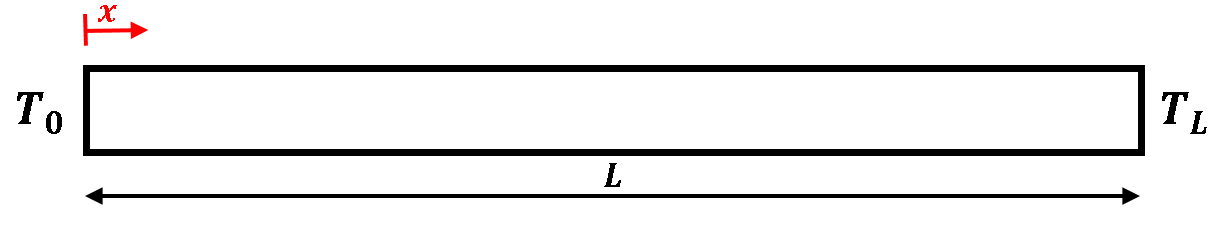
\includegraphics[width=14.00cm]{Chapter_2/figure/benchmark_case.png}
    \caption{One dimensional domain with heat conduction.}
    \label{fig:C2_benchmarkCase}
\end{figure}

The analytical solution for this problem is available and is written as shown in Equation \eqref{eq:C2_benchmarkCaseAnalyticalSolution}.

\begin{equation}\label{eq:C2_benchmarkCaseAnalyticalSolution}
    T = \frac{T_L - T_0}{L} x + T_0
\end{equation}

The analytical sensitivity of the temperature with respect to the beam's length is calculated by differentiating Equation \eqref{eq:C2_benchmarkCaseAnalyticalSolution} to $L$.

\begin{equation}
    \frac{\partial T}{\partial L} = -\frac{T_L - T_0}{L^2} x
\end{equation}

This is later used for verifying the discrete and continuous sensitivity results.

% -.-.-.-.-.-.-.-.-.-.-.-.-.-.-.-.-.-.-.-.-.-.-.-.-.-.-.-.-.-.-.-.-.-.-.-.-.-.-.-.-.-.-.
\subsection{Solid mechanics benchmark case}\label{section:C2_solid_mechanics_benchmark}
The axial bar is shown in Figure \ref{fig:C2_axialBarPhysicalShape}. The length of the bar is selected as $L = 1$ with axial stiffness of $EA = 1$. The distributed load is selected as a sine wave, $F_d(x) = sin(\pi x/L)$, with an extra axial load at the end, $F_p = 1 / \pi$. The beam is fixed using a spring of stiffness, $k = 10$, at $x = L$.

\begin{figure}[h]
    \centering
    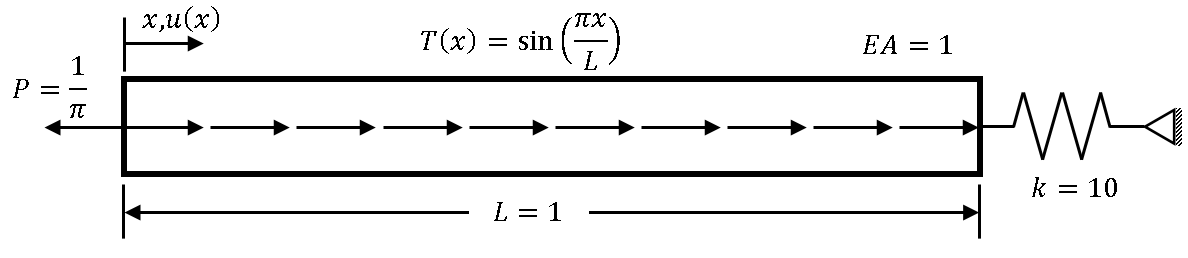
\includegraphics[width=14.00cm]{Chapter_2/figure/solid_mechanics_benchmark.png}
    \caption{Axial bar under distributed loading.}
    \label{fig:C2_axialBarPhysicalShape}
\end{figure}

The governing equation for the displacement of the axial bar and its corresponding boundary conditions are defined in Equation \eqref{eq:C2_axialBarGEandBC}. The bar length is selected as the design variable; therefore, it is included explicitly in the governing equation and boundary condition definitions.

\begin{subequations}
\begin{equation}\label{eq:C2_axialBarGE}
    \frac{\partial^2 u}{\partial x^2} + \sin \left( \frac{\pi}{L} x \right) = 0
\end{equation}
\begin{equation}\label{eq:C2_axialBarBC}
    \begin{cases}
    \dfrac{\partial u}{\partial x} \bigg|_{x = 0} = \dfrac{1}{\pi} \\
    \dfrac{\partial u}{\partial x} \bigg|_{x = L} = -10 u(L)
    \end{cases}
\end{equation}
\end{subequations}\label{eq:C2_axialBarGEandBC}

For this problem, the analytical solution is written as shown in Equation \eqref{eq:C2_axialBarSolution}.

\begin{equation}\label{eq:C2_axialBarSolution}
    u(x; L) = 
    \frac{L^2}{\pi^2} \sin \left( \frac{\pi x}{L} \right) + 
    \frac{2L + 10(L - 1)(L - x) - 1}{10 \pi}
\end{equation}

The displacement equation of \eqref{eq:C2_axialBarSolution} is differentiated to calculate the sensitivity of displacement to the length of the bar. The sensitivity equation \eqref{eq:C2_axialBarSensitivitySolution} is later used to verify the results of continuum and discrete sensitivity formulations.

\begin{equation}\label{eq:C2_axialBarSensitivitySolution}
    \dfrac{\partial u}{\partial L} = 
    \dfrac{2L}{\pi^2} \sin \left( \frac{\pi x}{L} \right) - 
    \dfrac{x}{\pi} \cos \left( \frac{\pi x}{L} \right) + 
    \dfrac{10L - 5x - 4}{5 \pi}
\end{equation}
% ======================================================================================
\section{Discrete Sensitivity Formulation}
The derivation of the discrete sensitivity equations starts with the discrete form of the governing equations. For the linear case, the governing equation \eqref{eq:C2_generalGoverningEquation} is discretized as shown in Equation \eqref{eq:C2_discreteGoverningEquation}

\begin{equation}\label{eq:C2_discreteGoverningEquation}
	\left[ K \right] \left[ U \right] = \left[ F \right]
\end{equation}

where $[K]$ is the discrete operator that represents the governing equation, $[U]$ is the vector of response variables defined at each of the degrees of freedom, and $[F]$ is the vector of the applied loads. The sensitivity of this system with respect to design variable $b$ is derived by differentiating Equation \eqref{eq:C2_discreteGoverningEquation}.

\begin{equation}\label{eq:C2_discreteSensitivityEquation}
	\left[ K \right] \left[ \frac{\partial U}{\partial b} \right] = 
	\left[ \frac{\partial F}{\partial b} \right] - 
	\left[ \frac{\partial K}{\partial b} \right] \left[ U \right]
\end{equation}

Solving Equation \eqref{eq:C2_discreteSensitivityEquation} yields a solution for sensitivity of response variable, $\partial u/\partial b$. This is achievable if the values of $\partial F/\partial b$ and $\partial K/\partial b$ are known. It should be noted that $U$ is a known value by the governing equation \eqref{eq:C2_discreteGoverningEquation} is solved. For the case of design independent loads, $\partial F/\partial b$ is equal to zero. This happens in many situations such as design optimization with pure mechanical loads. This assumption is violated for the cases when changing the design variables alter the loadings on the structure. The best example for this case is design of thermally loaded structures where due to thermal expansions, changing the size of elements will affect the thermal loadings \cite{deaton2013stiffening}. Calculating the $\partial K/\partial b$ term requires a detailed understanding about the discretization approach. This often requires source code modification which makes this method difficult to implement for commercial codes such as ABAQUS or FLUENT. The discrete method is highly accurate approach for calculating the sensitivities as will demonstrated with the following examples however, it is almost impossible to impliment in general purpose solvers.

% -.-.-.-.-.-.-.-.-.-.-.-.-.-.-.-.-.-.-.-.-.-.-.-.-.-.-.-.-.-.-.-.-.-.-.-.-.-.-.-.-.-.-.-.-.-
\subsection{Implementation for heat transfer}
The discrete sensitivity equations are formulated by discretizing the governing equation \eqref{eq:C2_laplaceEquation} using finite difference method. It should be noted that the finite difference is used for discretization of continuum governing equation and not for sensitivity calculation. Other techniques such as finite volume or finite elements can be used for the discretization of the governing equations as well. For this problem, the design variable affects the shape of the domain which is related to the distance between the nodes in the discrete manner. Therefore, for the sake of sensitivity analysis it is required to keep the nodal distances in the discretized solution as well. The domain is discretized by using 6 nodes as shown in Figure \ref{fig:C2_discretizedDomain}.

\begin{figure}[h]
	\centering
	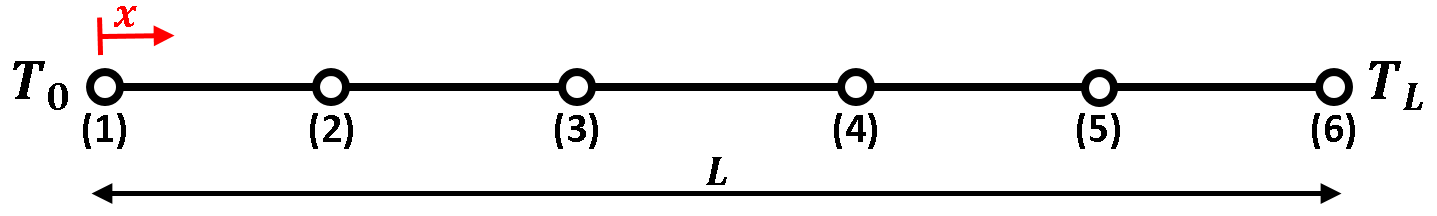
\includegraphics[width=14.00cm]{Chapter_2/figure/benchmark_case_computational_domain.png}
	\caption{One dimensional computational domain for the heat conduction problem.}
	\label{fig:C2_discretizedDomain}
\end{figure}

The second derivative of Equation \eqref{eq:C2_laplaceEquation} needs to be approximated for discretization. This is done by writing the Taylor series expansion of temperature at arbitrary location $x_i$. By using the central difference method the second order approximation for the second order derivative is written as shown in Equation \eqref{eq:C2_finiteDifferenceSchemes}.

To maintain the generality, we assume that distance of node $T_i$ to $T_{i+1}$ is $\Delta_i$ and the distance of node $T_i$ to $T_{i-1}$ is $\Delta_{i-1}$.

\begin{equation}\label{eq:C2_finiteDifferenceSchemes}
	\frac{\partial^2 T}{\partial x^2} = 
	\frac{T_{i-1} \Delta_{iL} - 
	      T_{i} (\Delta_{iL} + \Delta_{iR}) + 
	      T_{i+1} \Delta_{iR}}
	     {\dfrac{1}{2} \left[ \Delta_{iL} \Delta_{iR}^2 + 
	                         \Delta_{iL}^2 \Delta_{iR} \right]}
\end{equation}

The discretized governing equation of \eqref{eq:C2_finiteDifferenceSchemes} is written in a matrix form as shown in Equation \eqref{eq:C2_laplaceEquationMatrixForm}.

\begin{equation}\label{eq:C2_laplaceEquationMatrixForm}
	\begin{bmatrix}
		\frac{-2}{\Delta_{1} \Delta_{2}} &
		\frac{2}{\Delta_{1} \Delta_{2} + \Delta_{1}^2} &
		0 &
		0 &
		\\
		\frac{2}{\Delta_{3}^2 + \Delta_{2} \Delta_{3}} & 
		\frac{-2}{\Delta_{2} \Delta_{3}} &
		\frac{2}{\Delta_{2} \Delta_{3} + \Delta_{2}^2} &
		0
		\\
		0 &
		\frac{2}{\Delta_{4}^2 + \Delta_{3} \Delta_{4}} & 
		\frac{-2}{\Delta_{3} \Delta_{4}} &
		\frac{2}{\Delta_{3} \Delta_{4} + \Delta_{3}^2} &
		\\
		0 &
		0 &
		\frac{2}{\Delta_{5}^2 + \Delta_{4} \Delta_{5}} & 
		\frac{-2}{\Delta_{4} \Delta_{5}}
	\end{bmatrix}
	\begin{bmatrix}
		T_2 \\
		T_3 \\
		T_4 \\
		T_5
	\end{bmatrix}
	=
	-\begin{bmatrix}
	 	\frac{2T_1}{\Delta_{2}^2 + \Delta_{1} \Delta_{2}} \\
 		0 \\
		0 \\
		\frac{2T_6}{\Delta_{5} \Delta_{4} + \Delta_{5}^2}
	\end{bmatrix}
\end{equation}

To verify the discretization process, we compare the analytical solution of this problem with the result of Equation \eqref{eq:C2_laplaceEquationMatrixForm} in Figure \ref{fig:C2_verificationOfSolver}. For this problem we choose $T_1 = 0$, $T_6 = 1$ as the boundary conditions, and $L = 1$.  As shown in this figure, the discrete and continuum results match very well for different number of nodes. This is done by comparing the absolute error between the analytical and approximate results as shown in Table \ref{table:C2_solutionError}.

\begin{figure}[H]
	\centering
	\subfigure[$n = 6$]
	{
	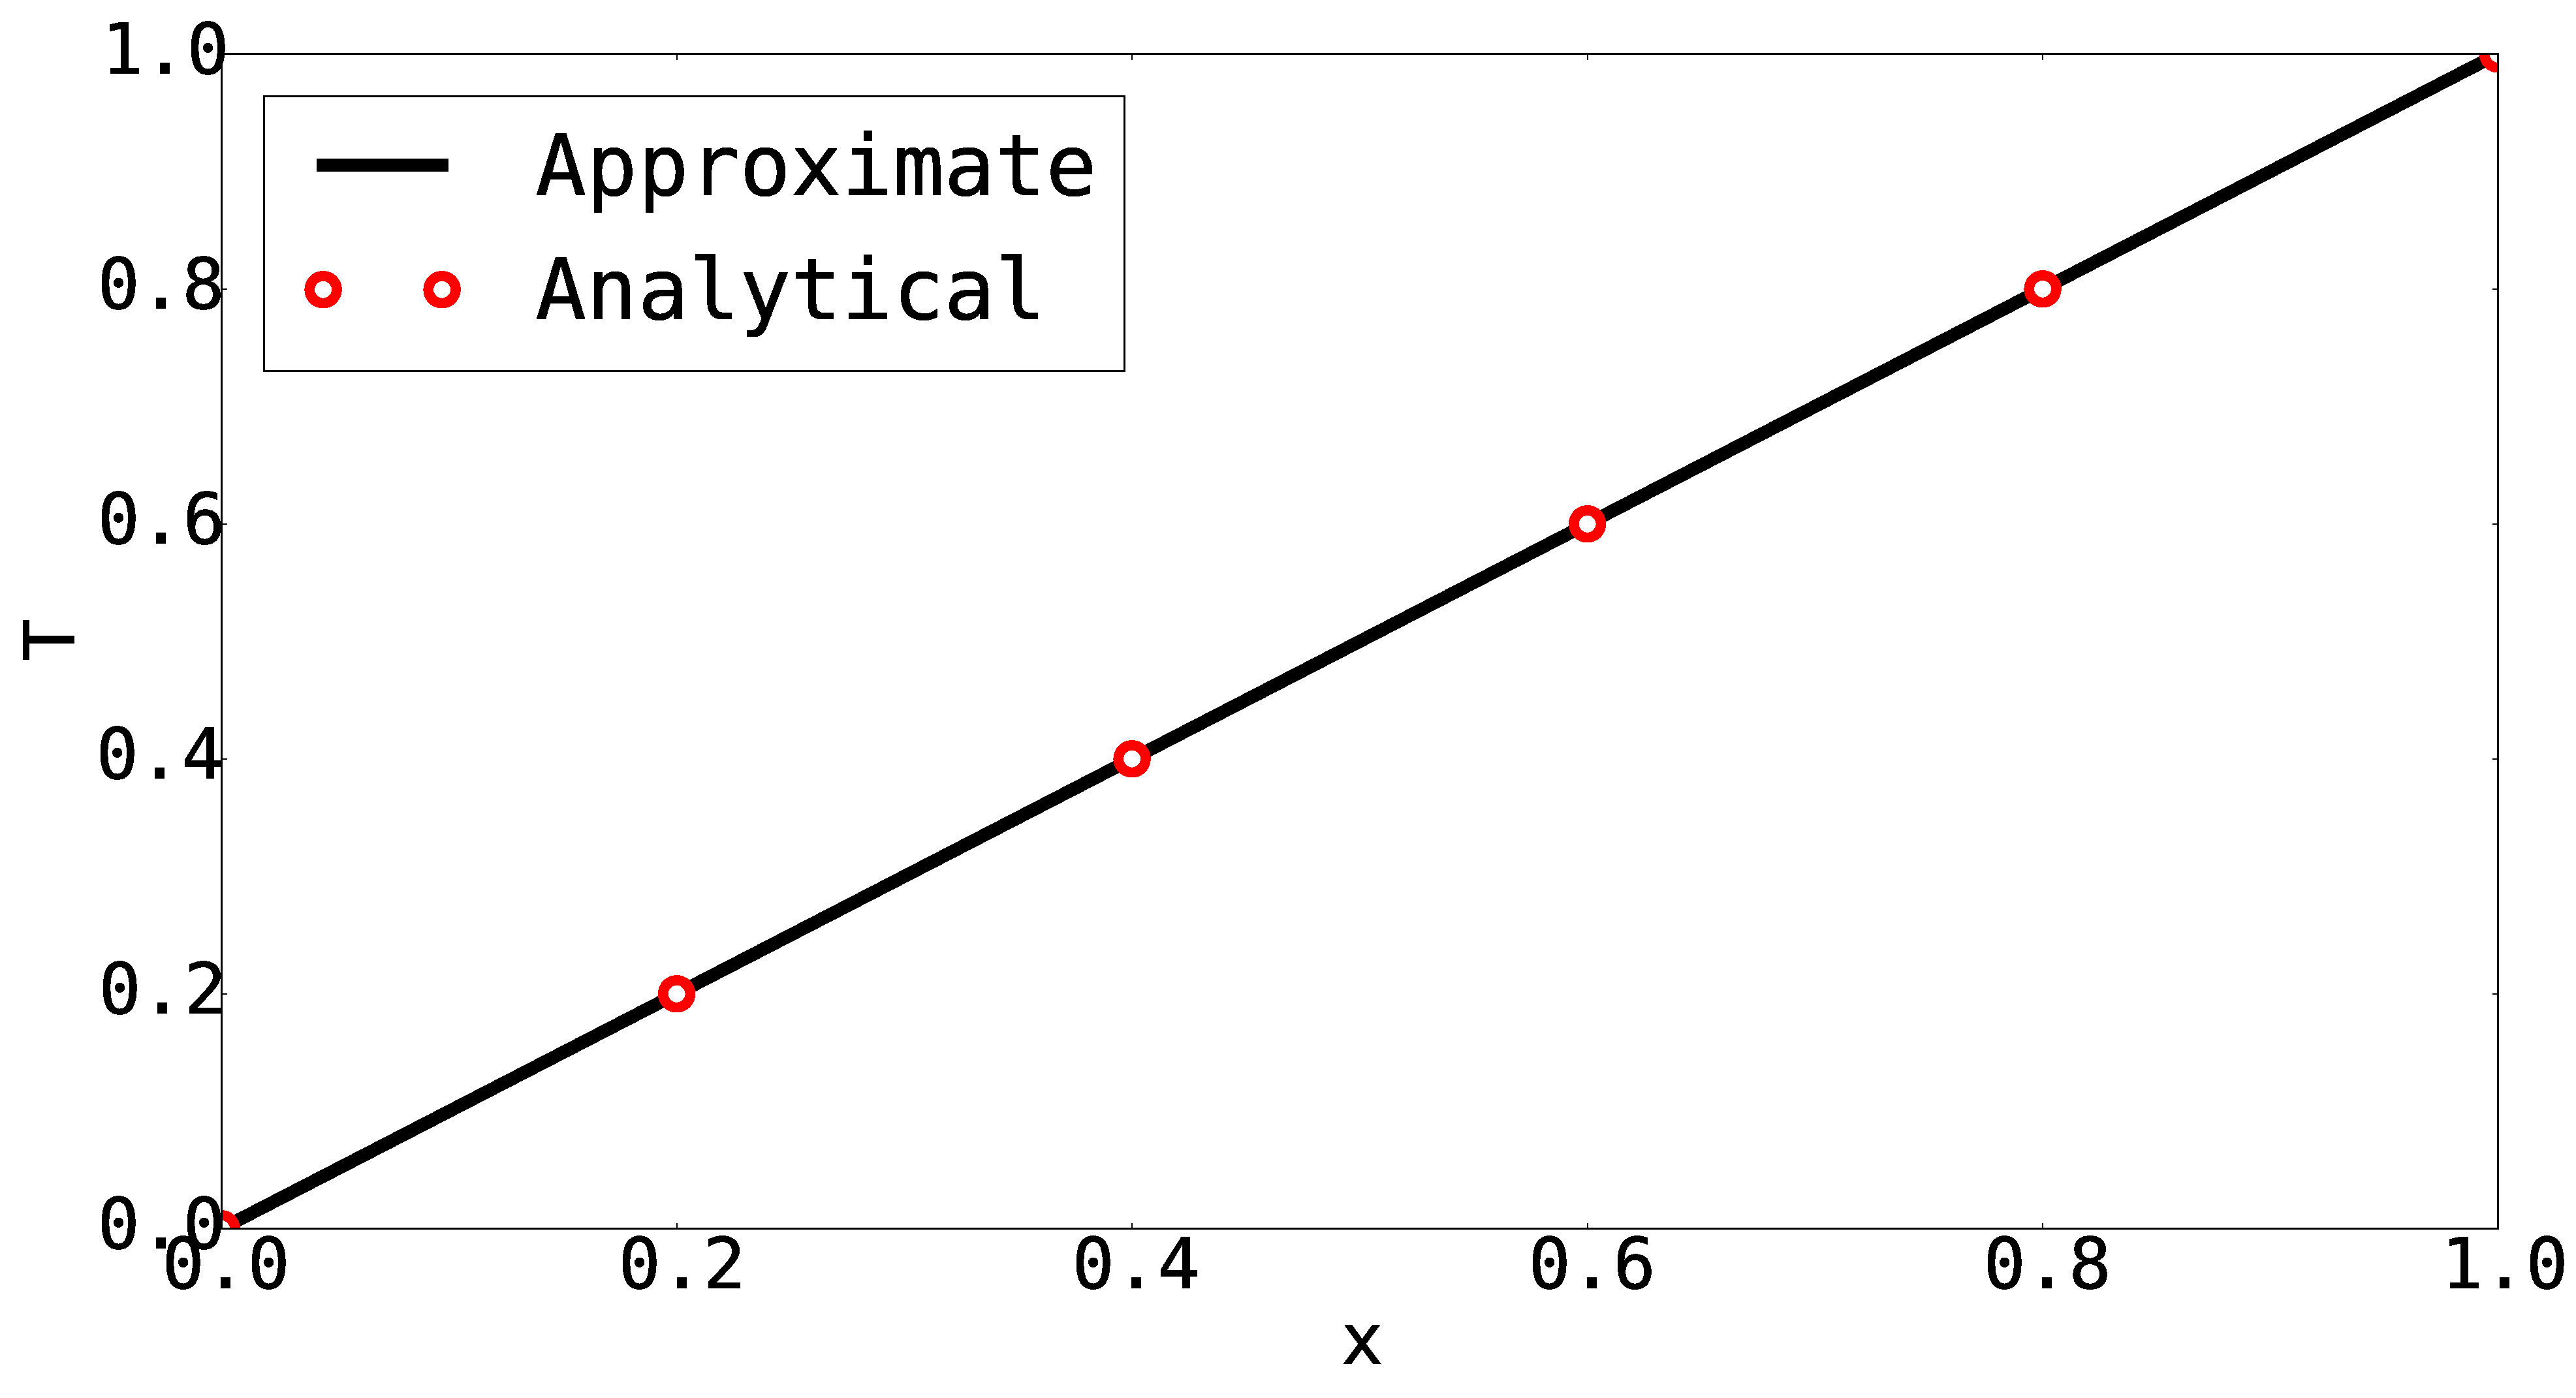
\includegraphics[width=7.0cm]{Chapter_2/figure/finitedifference_vs_analytical_n6.eps}
	}
	\quad
	\subfigure[$n = 12$]
	{
	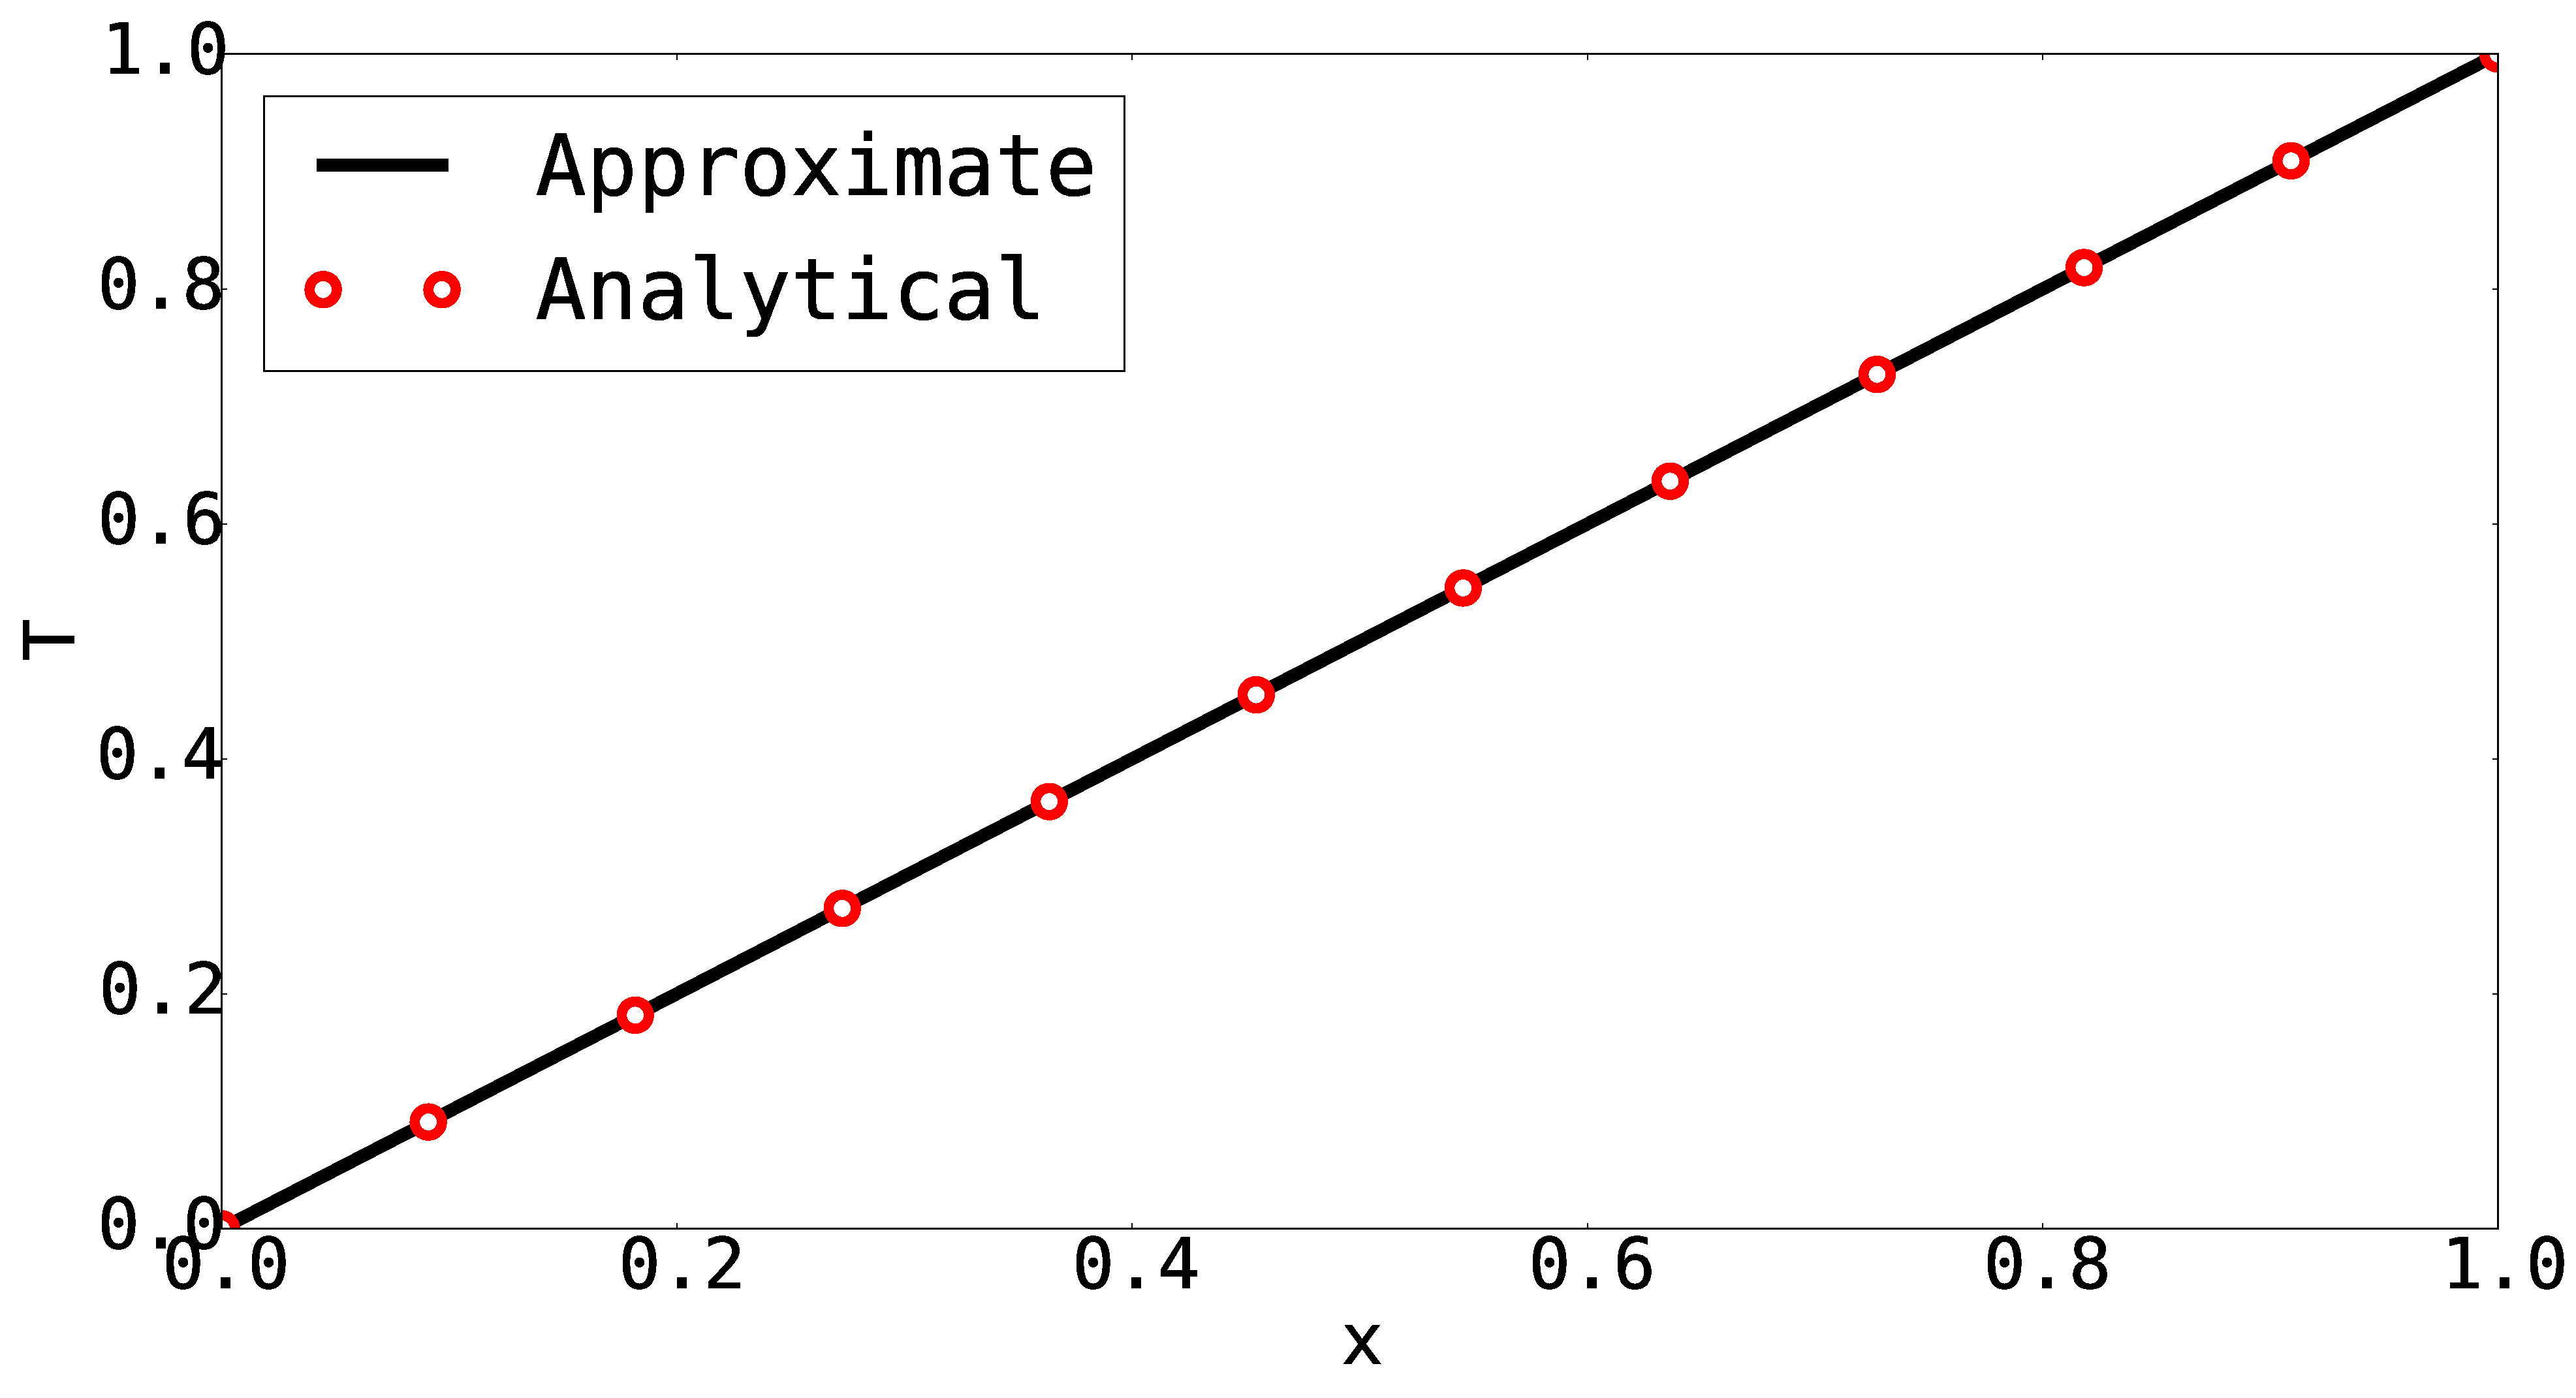
\includegraphics[width=7.0cm]{Chapter_2/figure/finitedifference_vs_analytical_n12.eps}
	}
	\\
	\subfigure[$n = 24$]
	{
	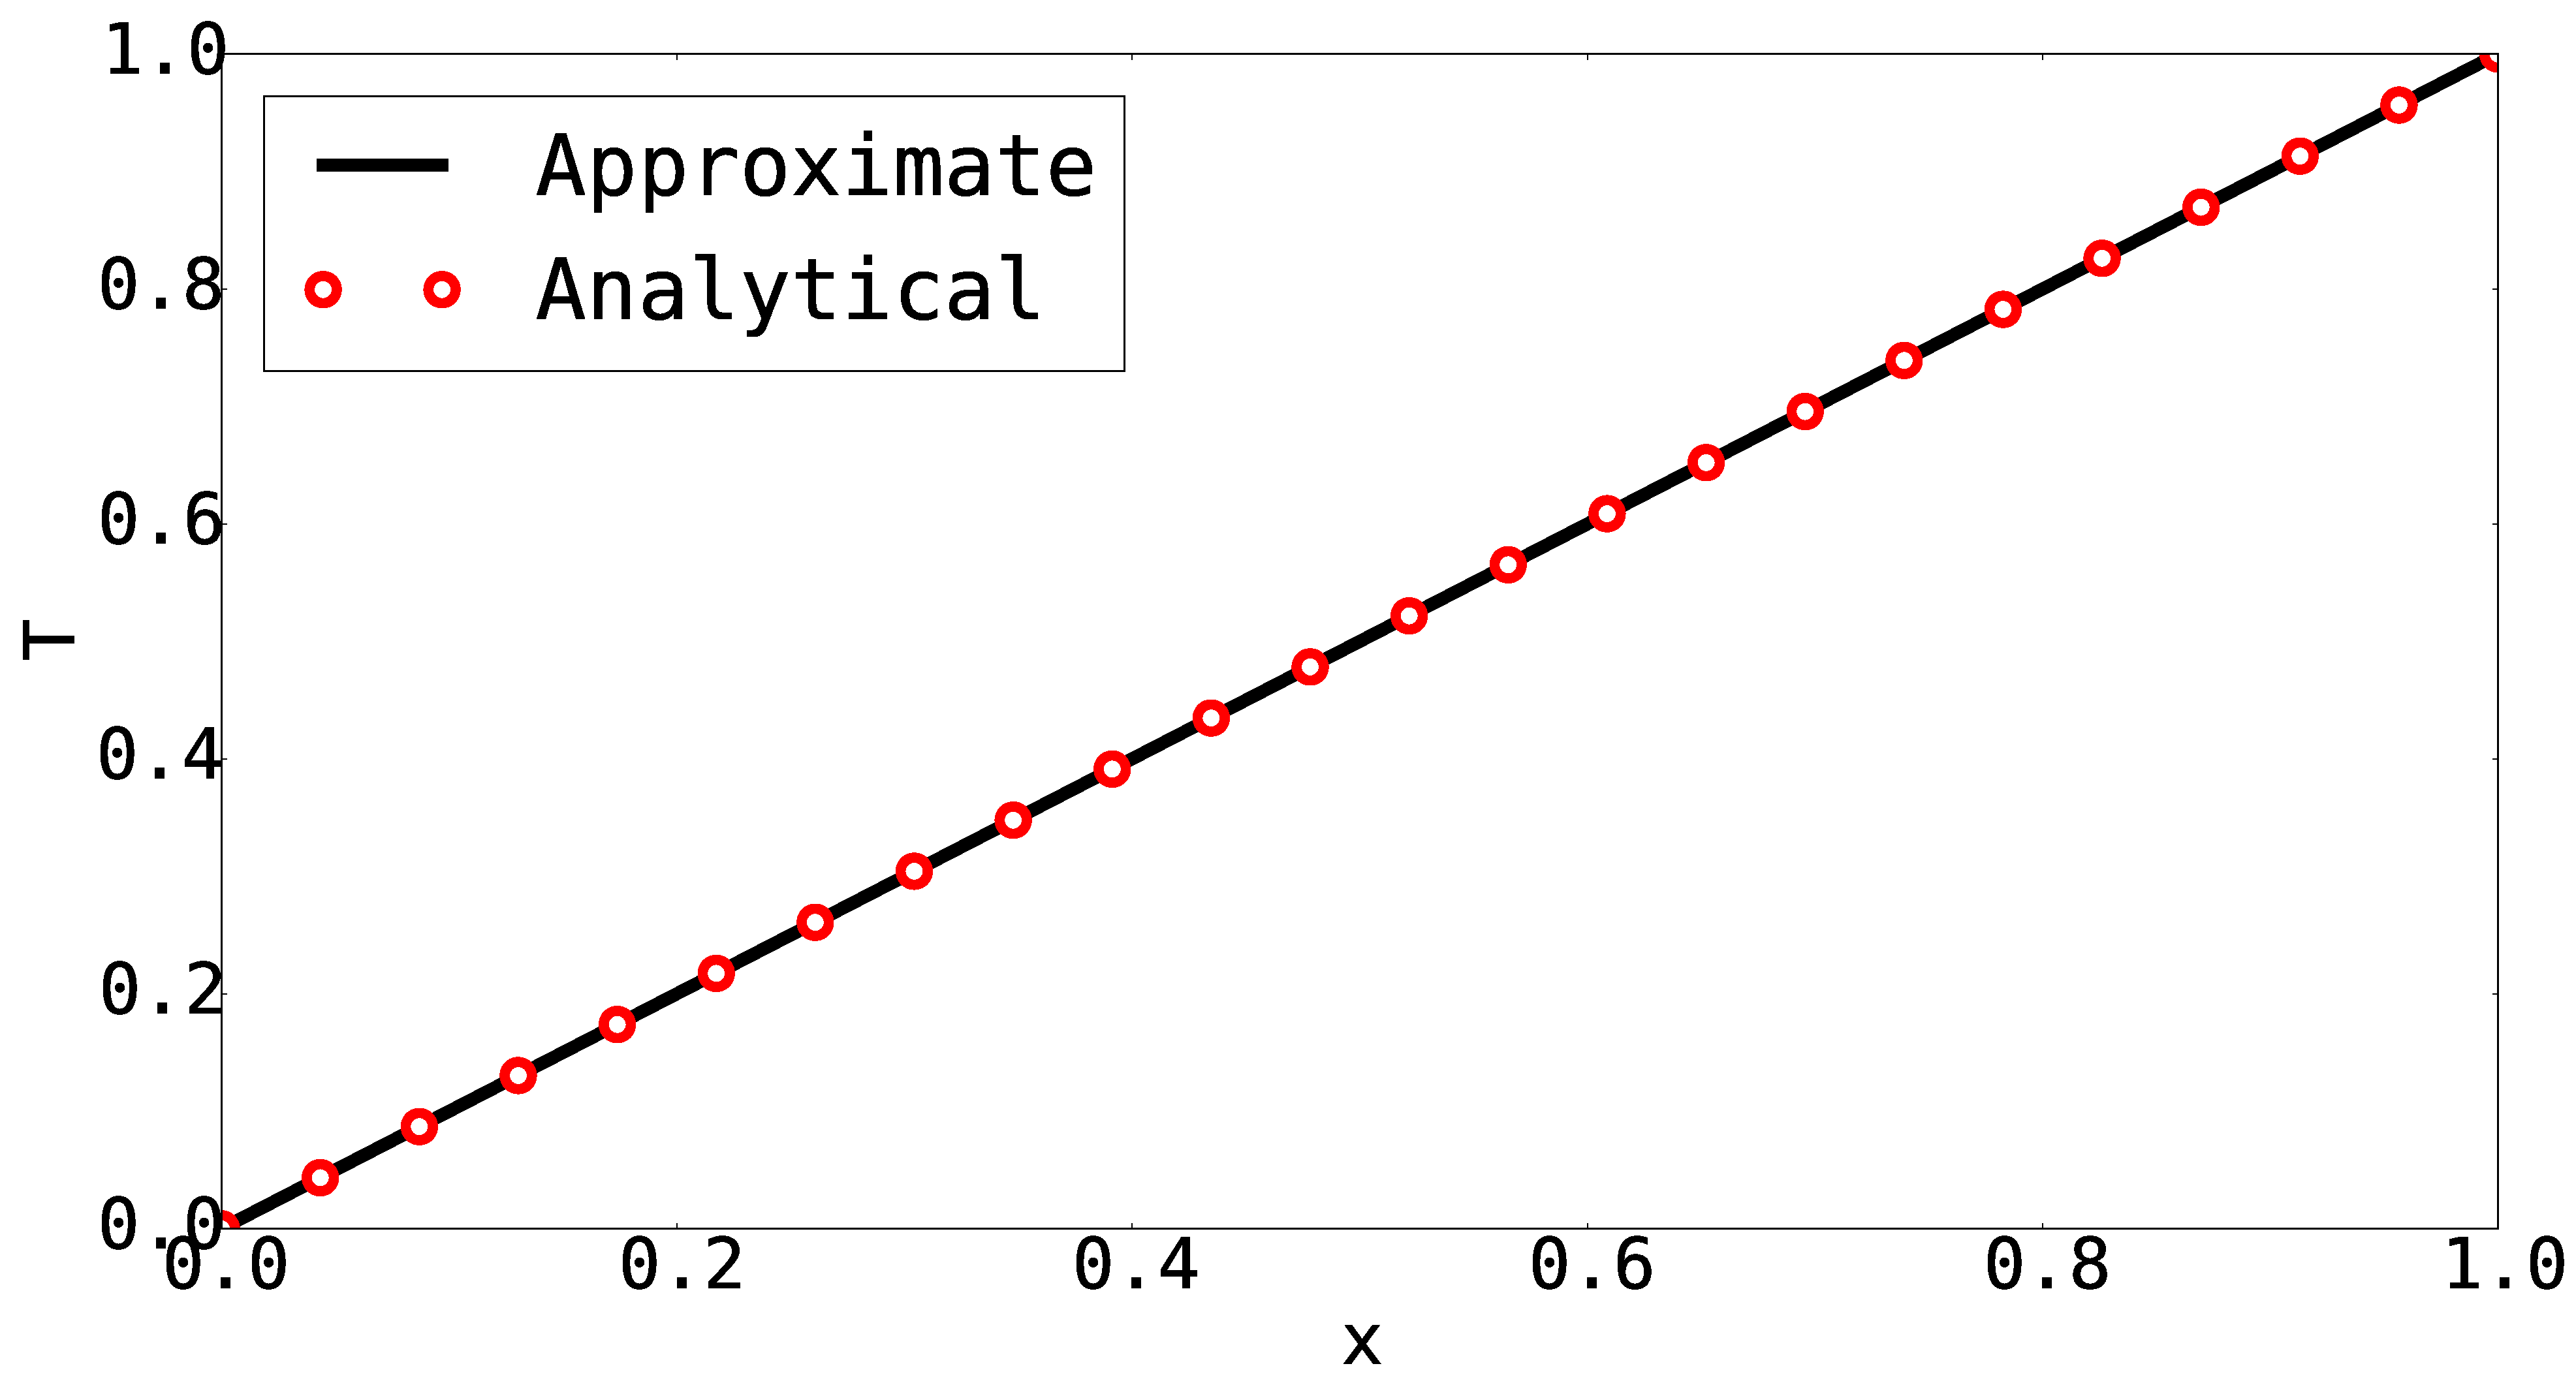
\includegraphics[width=7.0cm]{Chapter_2/figure/finitedifference_vs_analytical_n24.eps}
	}
	\quad
	\subfigure[$n = 48$]
	{
	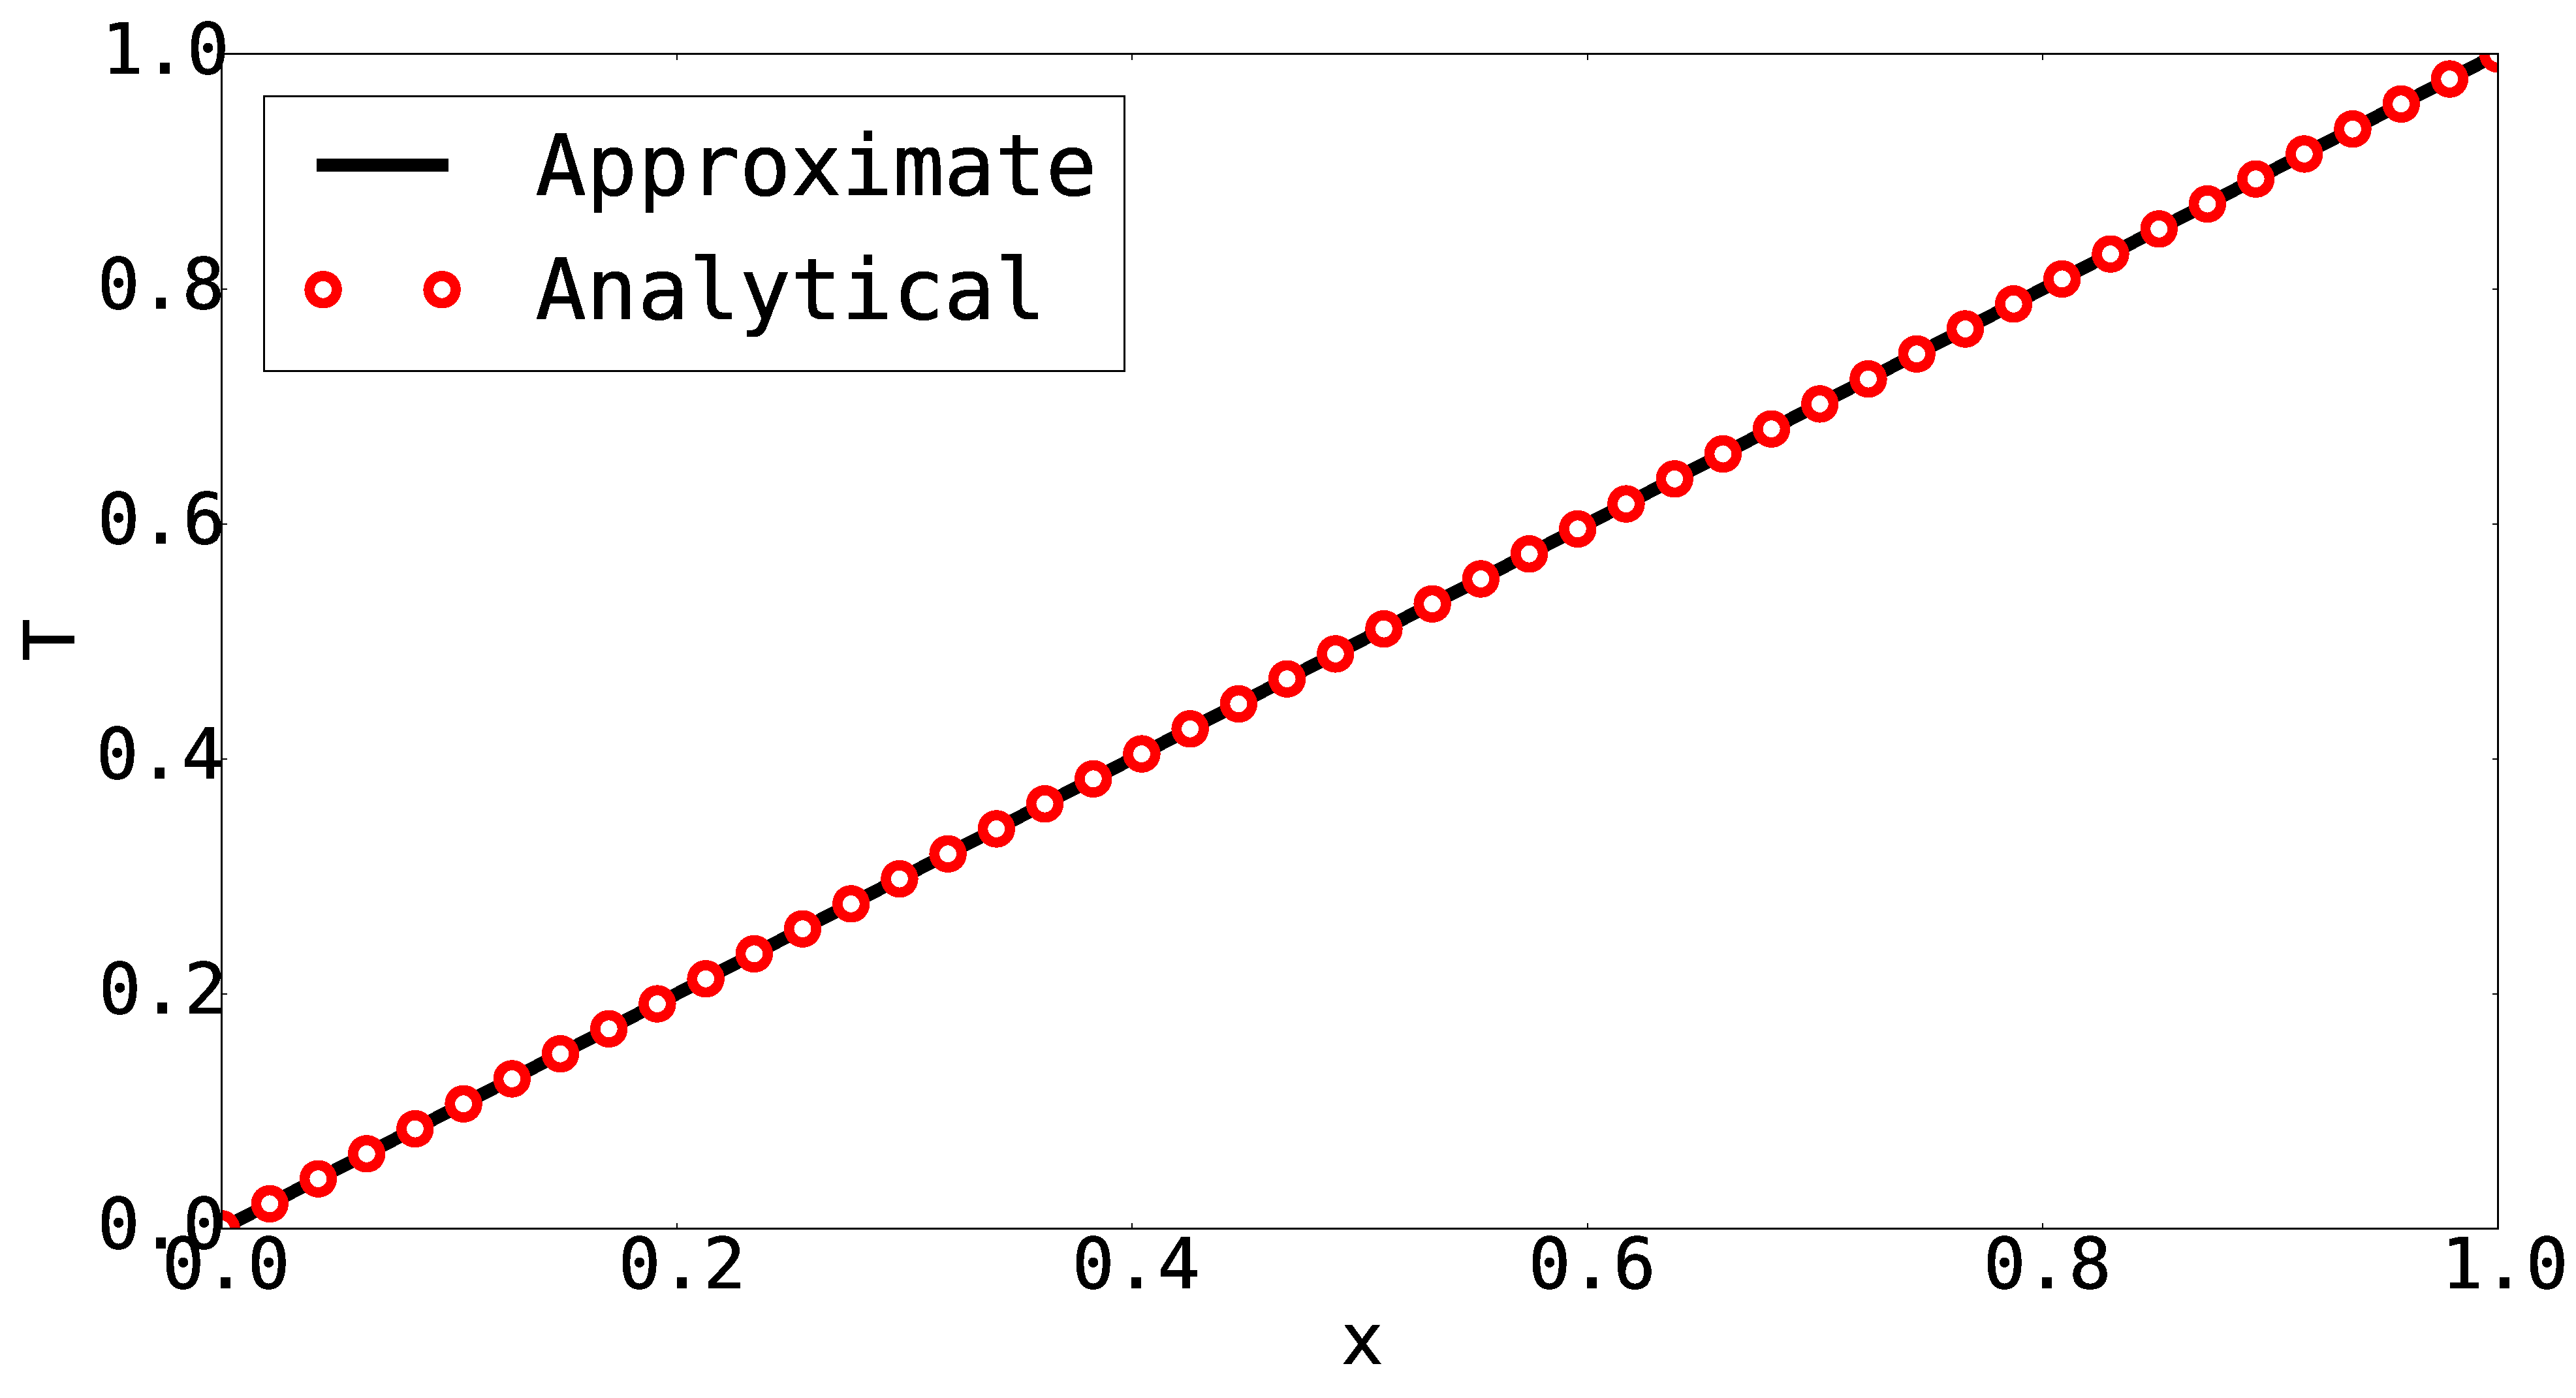
\includegraphics[width=7.0cm]{Chapter_2/figure/finitedifference_vs_analytical_n48.eps}
	}
	\caption{Comparison between the analytical and finite difference solutions for 1D heat equation for different number of nodes.}
	\label{fig:C2_verificationOfSolver}
\end{figure}

\begin{table}[H]
\centering
\begin{tabular}{| c | c |}
	\hline
	Number of nodes & absolute error \\ \hline \hline
	6 & $1.85 \times 10^{-16}$ \\ \hline
	12 & $2.03 \times 10^{-16}$ \\ \hline
	24 & $1.27 \times 10^{-15}$ \\ \hline
	48 & $8.55 \times 10^{-15}$ \\ \hline
\end{tabular}
\caption{Absolute error value for different number of nodes.}
\label{table:C2_solutionError}
\end{table}

The discrete sensitivity equations are derived by differentiating the discretized governing equation of \eqref{eq:C2_laplaceEquationMatrixForm} with respect to the length of the domain. We assume that the change in the length, only affects the nodal distance between the last two nodes and the rest remain unchanged. This means that only the node next to the boundary will move and the rest of nodes will be stationary. This is required to make sure that the sensitivity at each of the degrees of freedom is only a function of change in shape not movement of material nodes therefore, $\partial x/\partial b$ is equal to zero.

In order to differentiate Equation  \eqref{eq:C2_laplaceEquationMatrixForm}, it is required to calculate the derivative of nodal distances in Equation \eqref{eq:C2_laplaceEquationMatrixForm} with respect to $L$, $\partial \Delta_i/\partial L$. For an equally spaced grid, the nodal distance is written as

\begin{equation*}
	\Delta = \frac{L}{n - 1}
\end{equation*}

where $L$ is the length of the domain, and $n$ is the number of nodes used to discretize the domain. Therefore, the sensitivity of nodal distances to the length of the domain is calculated as

\begin{equation}\label{eq:C2_nodeDistanceSensitivity}
	\frac{\partial \Delta}{\partial L} = \frac{1}{n-1}
\end{equation}

The differentiated form of the discretized equation is written as shown in Equation \eqref{eq:C2_laplaceEquationMatrixFormSensitivity}. It should be noted that since only the adjacent node to the boundary is affected by shape change, only that element in the matrix derivative has a value.

\begin{equation}\label{eq:C2_laplaceEquationMatrixFormSensitivity}
	\begin{bmatrix}
		-2 & 1 & 0 & 0 \\
		1 & -2 & 1 & 0 \\
		0 & 1 & -2 & 1 \\
		0 & 0 & 1 & -2
	\end{bmatrix}
	\begin{bmatrix}
		T'_2 \\
		T'_3 \\
		T'_4 \\
		T'_5
	\end{bmatrix}
	=
	\frac{1}{2} \frac{\partial \Delta}{\partial L} \frac{1}{\Delta}
	\begin{bmatrix}
		0 \\
		0 \\
		0 \\
		T_6
	\end{bmatrix}
	-
	\underbrace{
	\frac{1}{2} \frac{\partial \Delta}{\partial L} \frac{1}{\Delta}
	\begin{bmatrix}
		0 & 0 & 0 & 0 \\
		0 & 0 & 0 & 0 \\
		0 & 0 & 0 & 0 \\
		0 & 0 & -3 & 1
	\end{bmatrix}
	\begin{bmatrix}
		T_2 \\
		T_3 \\
		T_4 \\
		T_5
	\end{bmatrix}}_\text{effect of shape change}
\end{equation}

where $T^\prime_i$ represents the sensitivity of temperature with respect to length of the domain.

To verify the results of Equation \eqref{eq:C2_laplaceEquationMatrixFormSensitivity}, we compared it with the analytical sensitivity results as shown in Figure \ref{fig:C2_discreteSensitivityVerification}. We discretized the domain using $11$, $41$, $81$, and $161$ nodes for this purpose, however this does not affect the solution accuracy. We chose the normalized root-mean-square deviation (NRMSD) for comparing the sensitivity results. This is defined as shown in Equation \eqref{eq:C2_NRMSD}.

\begin{equation}\label{eq:C2_NRMSD}
	NRMSD = \dfrac{\sqrt{\dfrac{\sum (\hat{y}_t - y)^2}{n}}}{y_{max} - y_{min}}
\end{equation}

where $\hat{y}$ is the value calculated using DSA and $y$ is the true value calculated by analytical equation. The results for the NRMSD for this problem for different number of nodes are shown in Table \ref{table:C2_DSA_NRMSD}.

\begin{figure}[H]
	\centering
	\subfigure[$n = 11$]
	{
	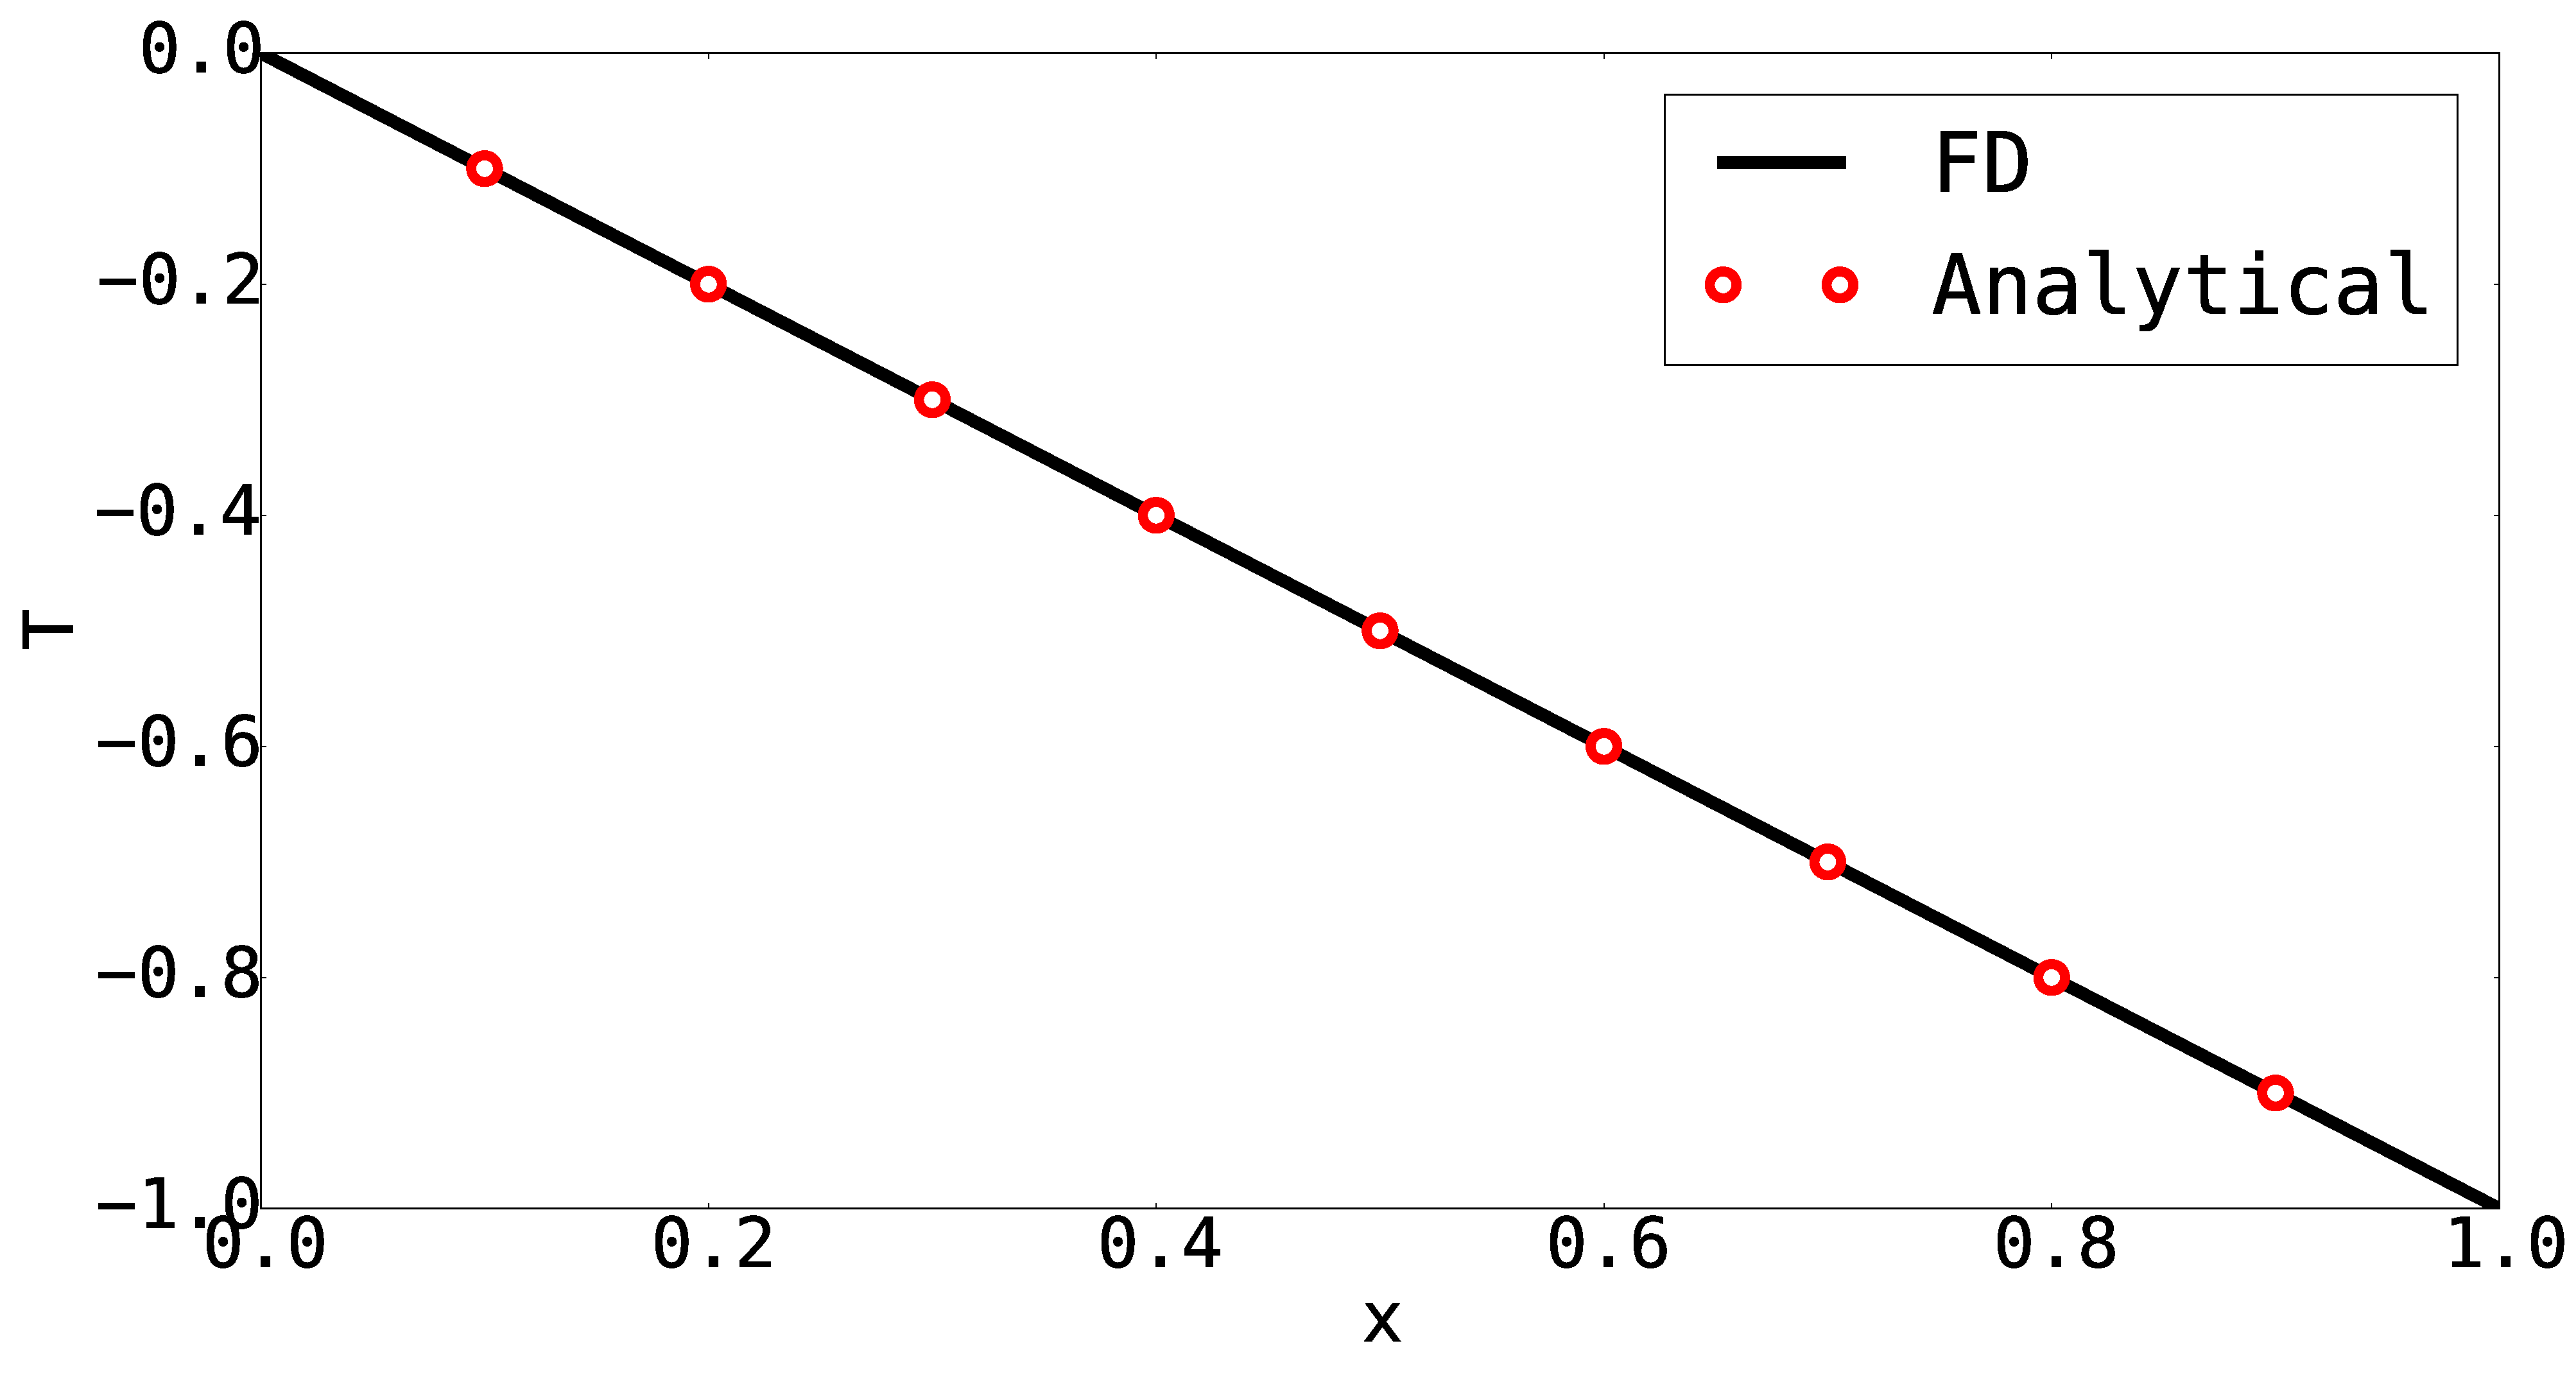
\includegraphics[width=7.0cm]{Chapter_2/figure/DSA_n11.eps}
	}
	\quad
	\subfigure[$n = 41$]
	{
	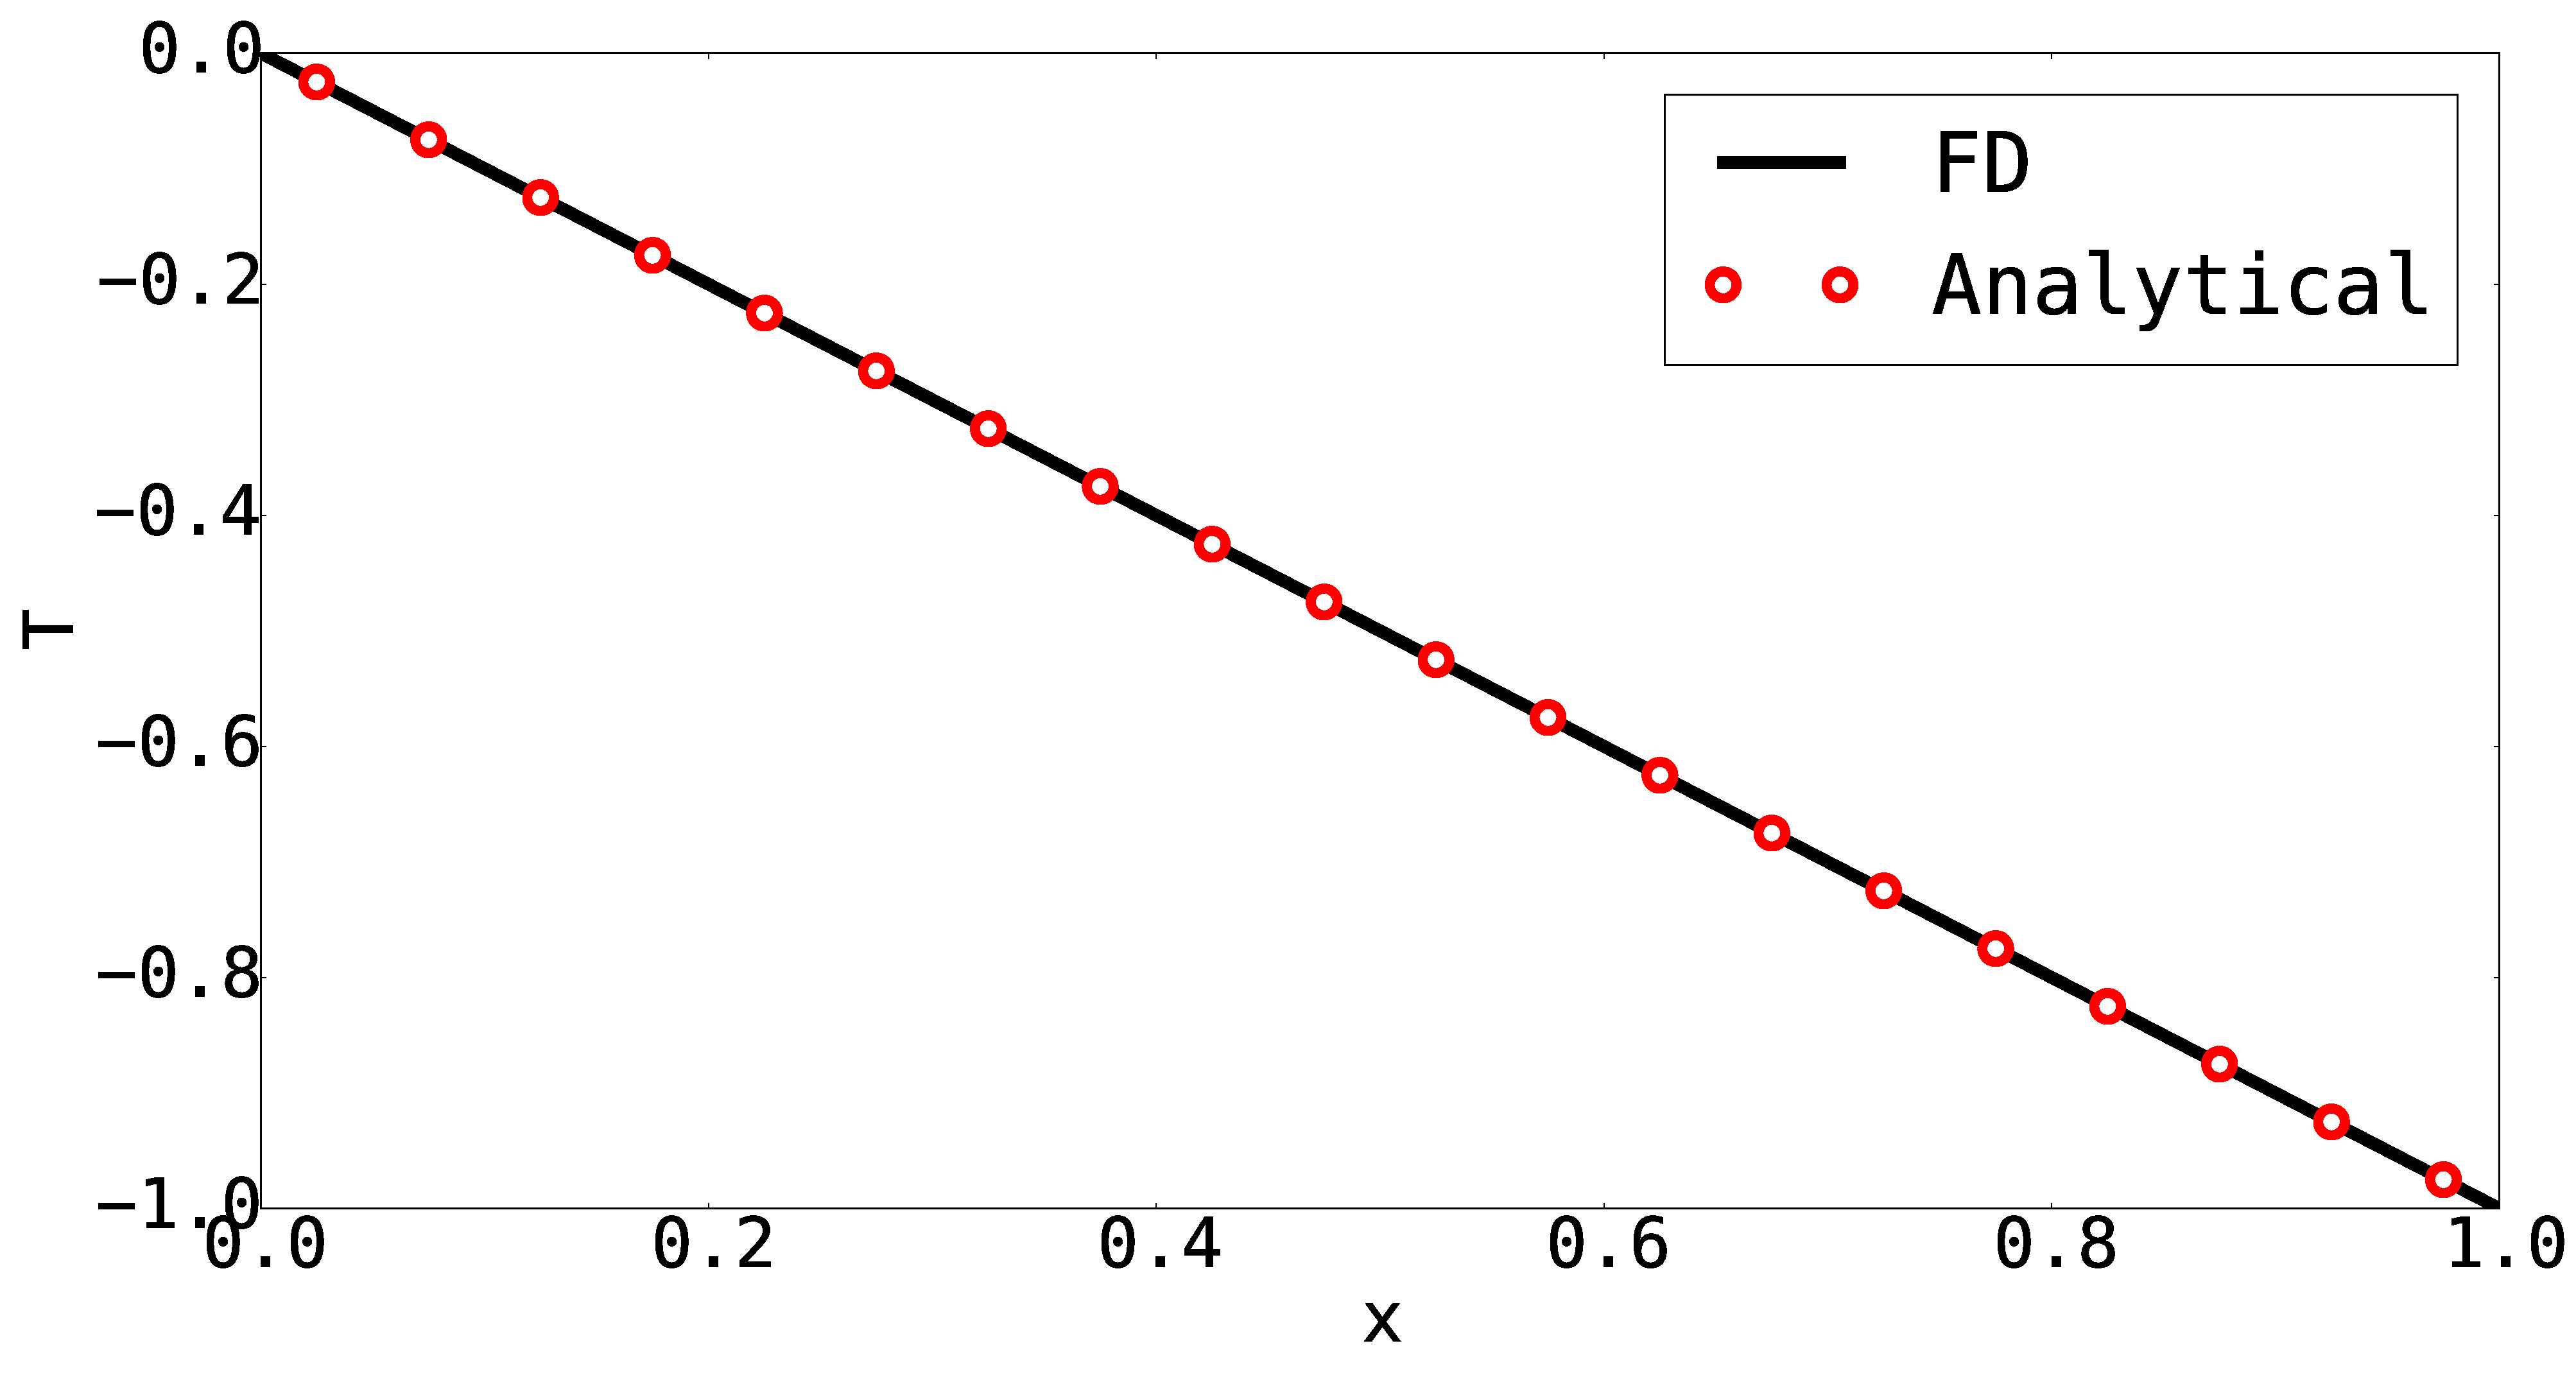
\includegraphics[width=7.0cm]{Chapter_2/figure/DSA_n41.eps}
	}
	\\
	\subfigure[$n = 81$]
	{
	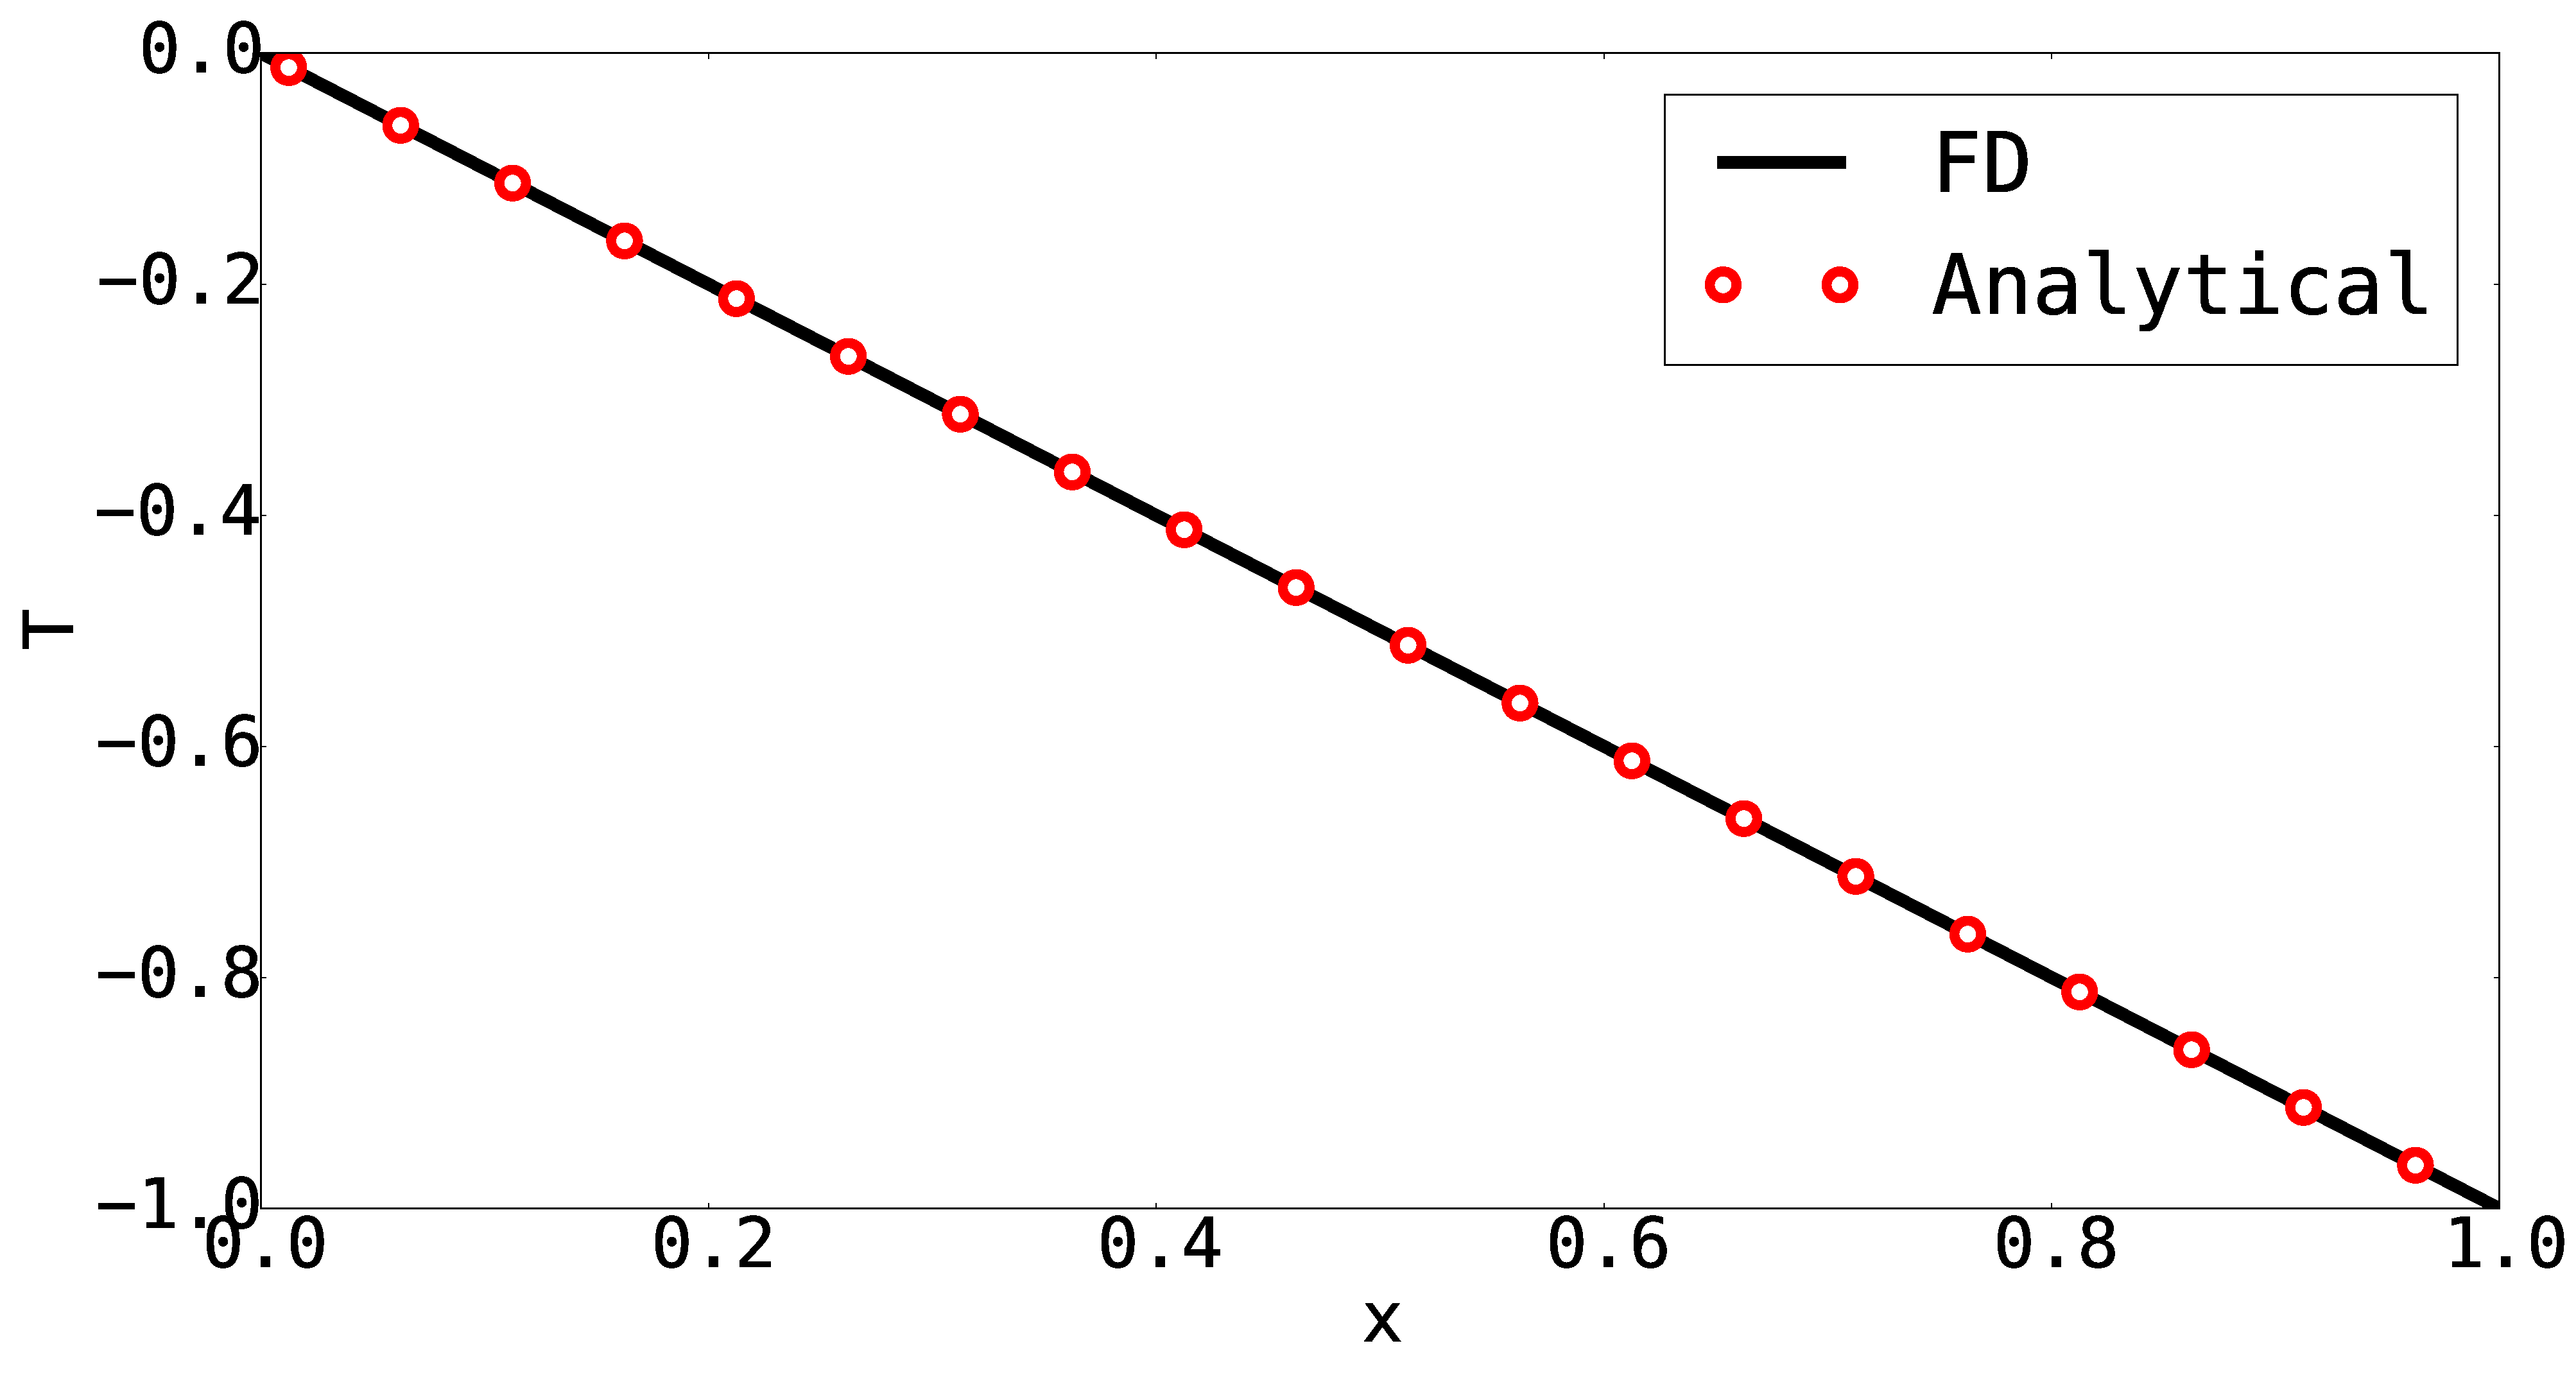
\includegraphics[width=7.0cm]{Chapter_2/figure/DSA_n81.eps}
	}
	\quad
	\subfigure[$n = 161$]
	{
	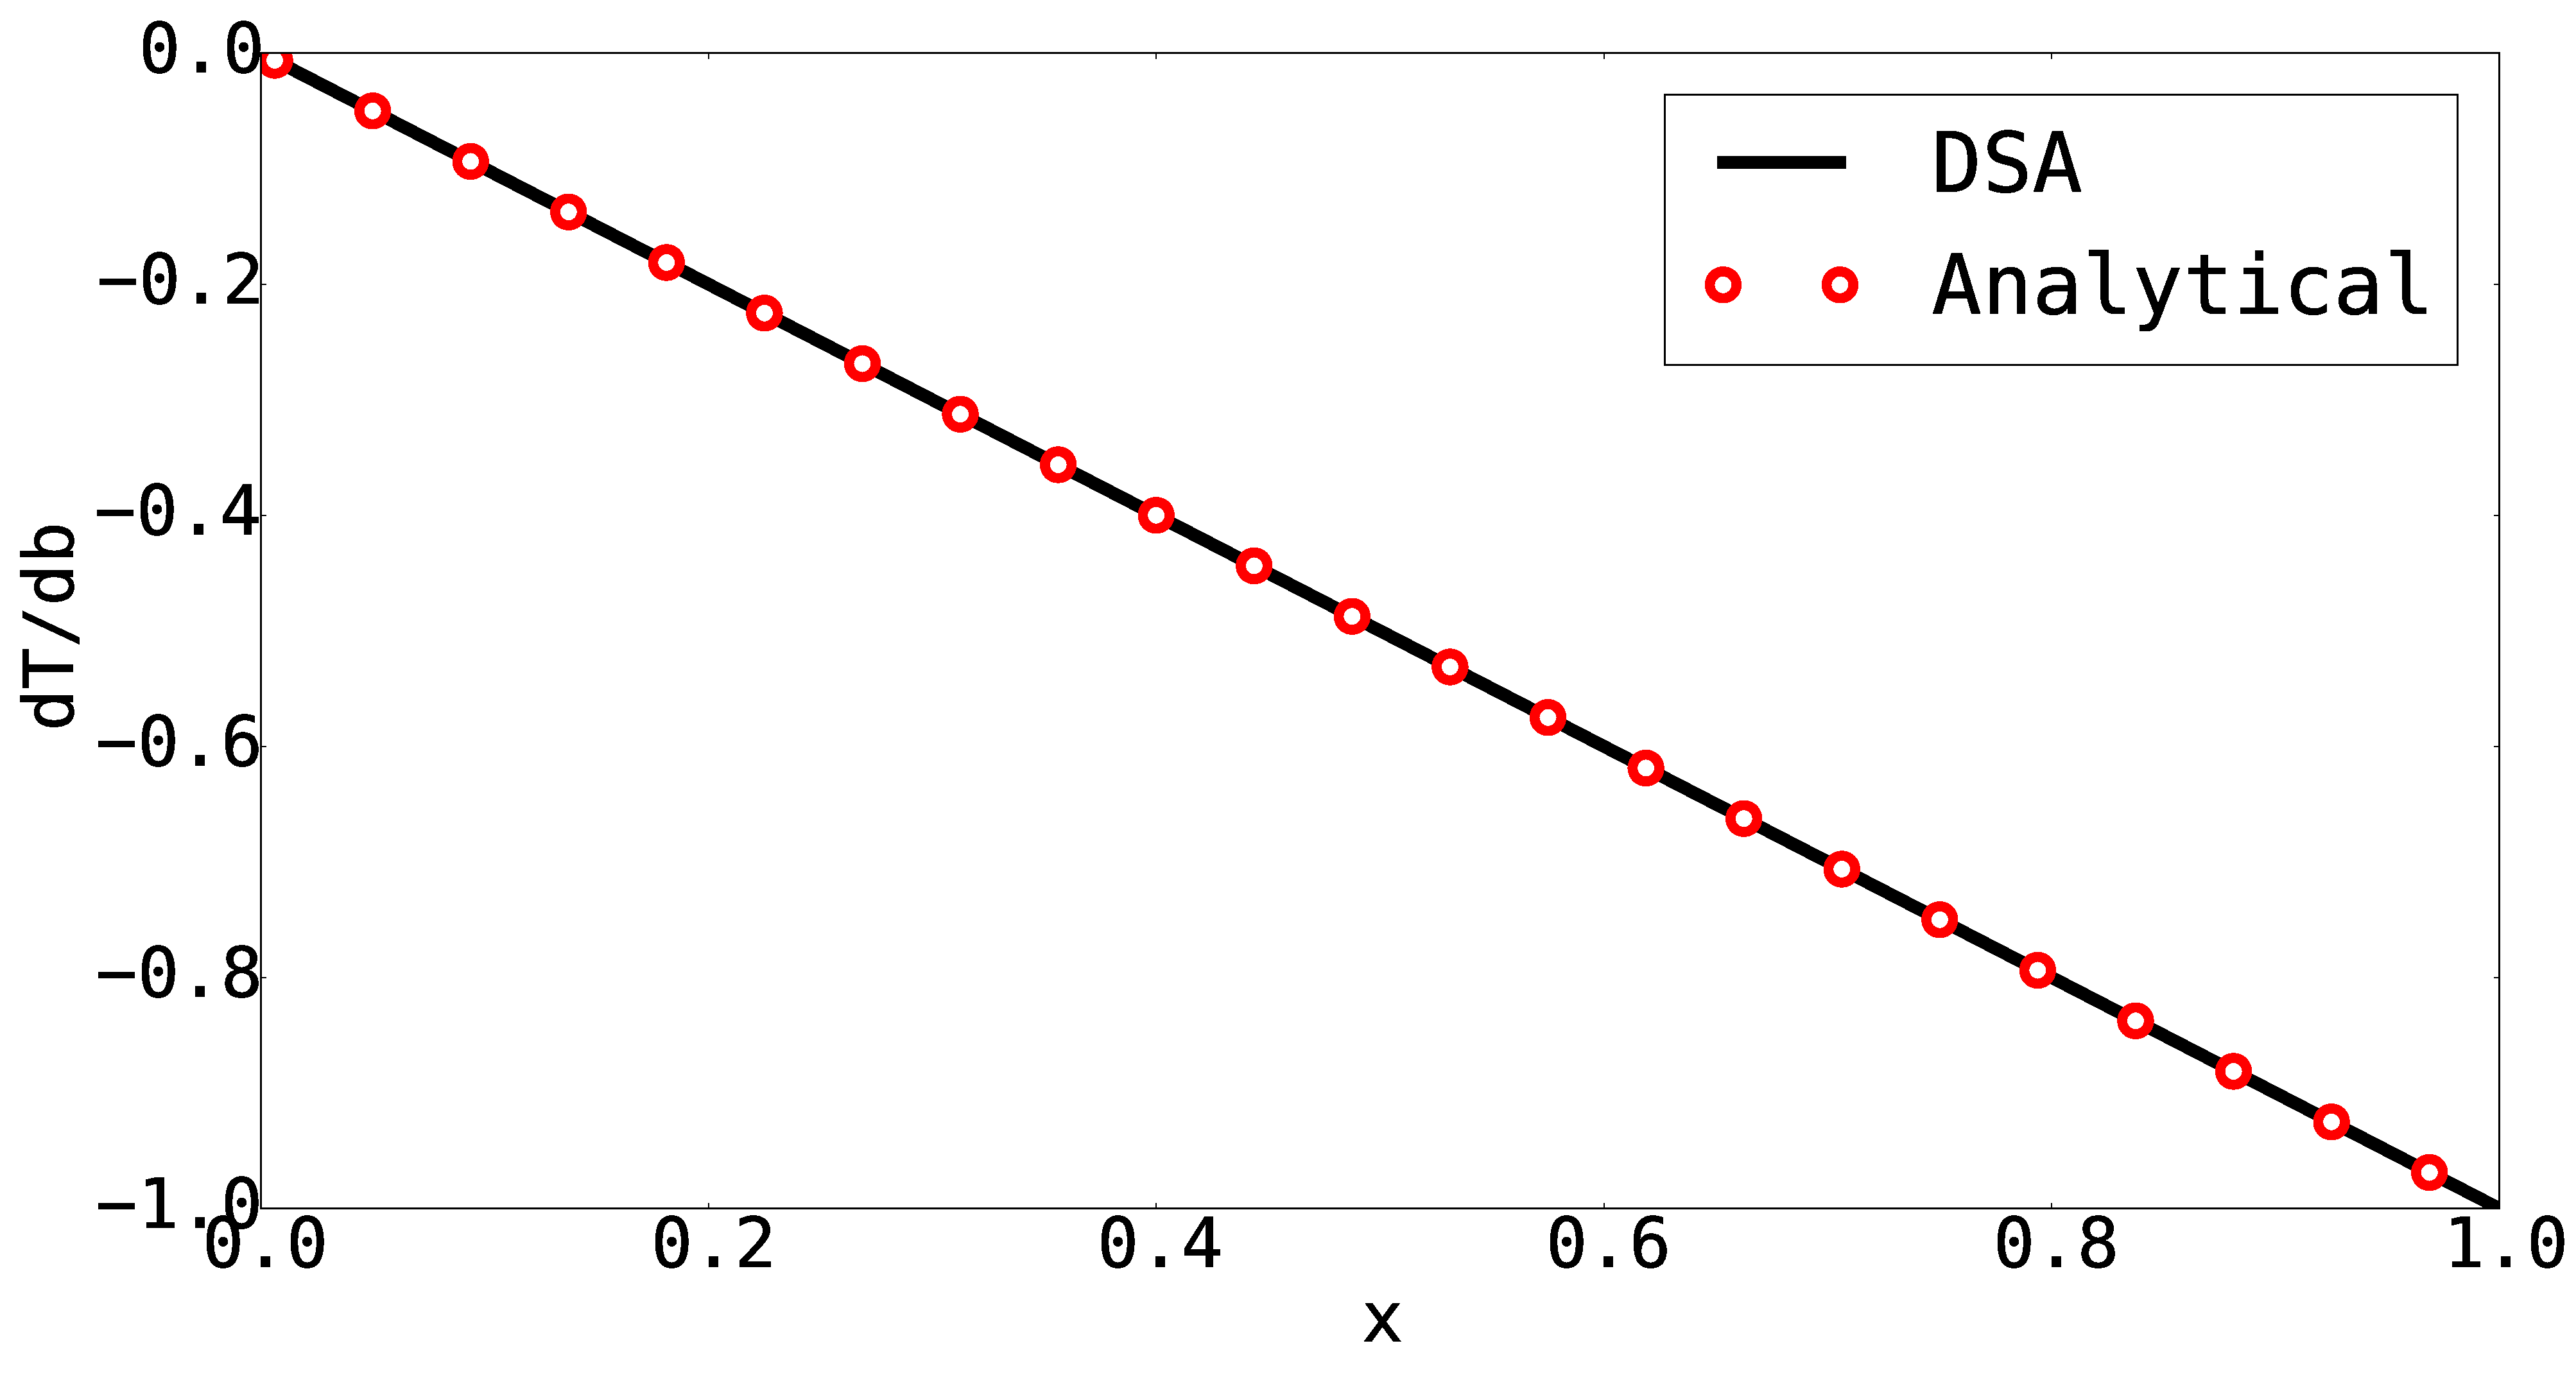
\includegraphics[width=7.0cm]{Chapter_2/figure/DSA_n161.eps}
	}
	\caption{Comparison between discrete sensitivity analysis and analytical results for different number of nodes.}
	\label{fig:C2_discreteSensitivityVerification}
\end{figure}

\begin{table}[H]
\centering
\begin{tabular}{| c | c |}
	\hline
	Number of nodes & NRMSD \\ \hline \hline
	11 & $1.68 \times 10^{-16}$ \\ \hline
	41 & $2.49 \times 10^{-15}$ \\ \hline
	81 & $1.49 \times 10^{-15}$ \\ \hline
	161 & $2.85 \times 10^{-15}$ \\ \hline
\end{tabular}
\caption{RMSE value for different number of nodes.}
\label{table:C2_DSA_NRMSD}
\end{table}

As shown in Figure \ref{fig:C2_discreteSensitivityVerification} and Table \ref{table:C2_DSA_NRMSD}, the accuracy of discrete sensitivity analysis is not affected by the number of nodes chosen to discretize the domain.

% -.-.-.-.-.-.-.-.-.-.-.-.-.-.-.-.-.-.-.-.-.-.-.-.-.-.-.-.-.-.-.-.-.-.-.-.-.-.-.-.-.-.-.-.-.-
\subsection{Implementation for solid mechanics problem}
Finite elements are used to discretized the axial bar problem shows in Figure \ref{fig:C2_axialBarPhysicalShape}. The governing equation of \eqref{eq:C2_axialBarGE} is discretized using a uniform mesh, linear shape functions, and point one point Gauss integration. As mentioned in Section \ref{section:C2_solid_mechanics_benchmark}, the design variable is selected as the length of the bar and it will affect the distances between the nodes. In order to keep the local and total derivatives equal, we fix the interior computational nodes in space and change the length of the bar by only moving the last node. Therefore, the shape design variable only affects the size of the last element and it should be included in the discretized equations. This is shown in Figure \ref{fig:C2_axialBarComputationalDomain}. Since the internal nodes do not move, the design velocity is zero for these nodes.

\begin{figure}[H]
	\centering
	\subfigure[Original domain.]
	{
	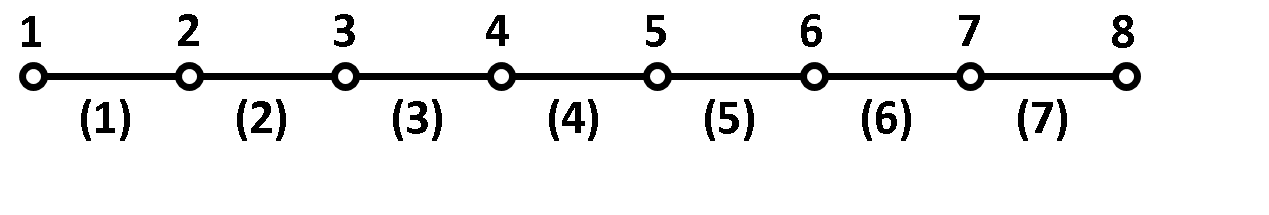
\includegraphics[width=14.0cm]{Chapter_2/figure/bar_computational_before.png}
	}
	\\
	\subfigure[Deformed domain.]
	{
	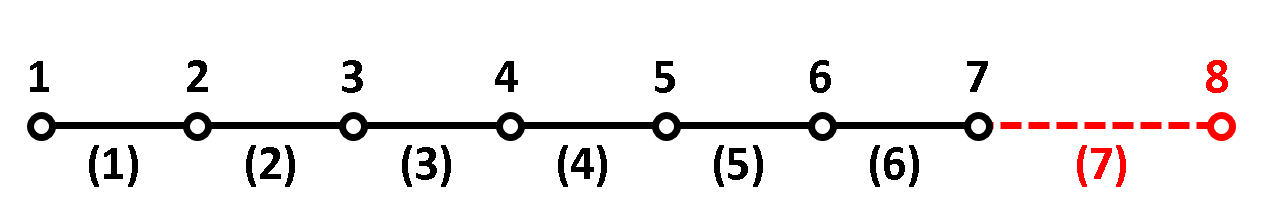
\includegraphics[width=14.0cm]{Chapter_2/figure/bar_computational_after.png}
	}
	\caption{Changing the length of bar by fixing the interior computational nodes and moving only the boundary (red) node. Node numbers are represented by $i$ and element numbers by $(i)$.}
	\label{fig:C2_axialBarComputationalDomain}
\end{figure}

For the case of three elements, the stiffness matrix is written as

\begin{equation}\label{eq:C2_stiffnessMatrixOfBar}
	[K] = 
	EA
	\begin{bmatrix}
	1/l_1 & -1/l_1 & 0 & 0 \\
	-1/l_1 & 1/l_1 + 1/l_2 & -1/l_2 & 0 \\
	0 & -1/l_2 & 1/l_2 + 1/l_3 & -1/l_3 \\
	0 & 0 & -1/l_3 & 1/l_3
	\end{bmatrix}
\end{equation}

where $l_i$ are the length of the elements. It should be noted that only $l_3$ is affected by changing the length of the domain in this formulation of the problem. The disretized equation for this problem is written as shown in Equation \eqref{eq:C2_discretizedBarEquation}.

\begin{equation}\label{eq:C2_discretizedBarEquation}
	[K - K_s] [U] = [F_d] - [F_p]
\end{equation}

where $[K]$ is the stiffness matrix of the bar, $[K_s]$ is the stiffness of the spring boundary, $[F_d]$ is the distributed load, and $[F_p]$ is the point load. The point load is substracted because of its negative direction for this problem. For the case of $EA = 1$, $F_d = \sin(\pi x / 2)$, $L = 1$, $P = 1 / \pi$ and $K_s = 10$ the solution of Equation \eqref{eq:C2_discretizedBarEquation} is compared with the analytical results of the problem as shown in Equation \eqref{eq:C2_axialBarSolution} in Figure \ref{fig:C2_axialBarSolution}. We chose Normalized Root-Mean-Square Deviation as the metric of comparison. This is calculated as shown in Equation \eqref{eq:C2_NRMSD_beam}

\begin{equation}\label{eq:C2_NRMSD_beam}
	NRMSD = \dfrac{\sqrt{\dfrac{\sum_{t=1}^n \left( \hat{y}_t - y \right)^2}{n}}}{y_{max} - y_{min}}
\end{equation}

where $\hat{y}_t$ is the numerical and $y$ is the analytical result.

\begin{figure}[h]
	\centering
	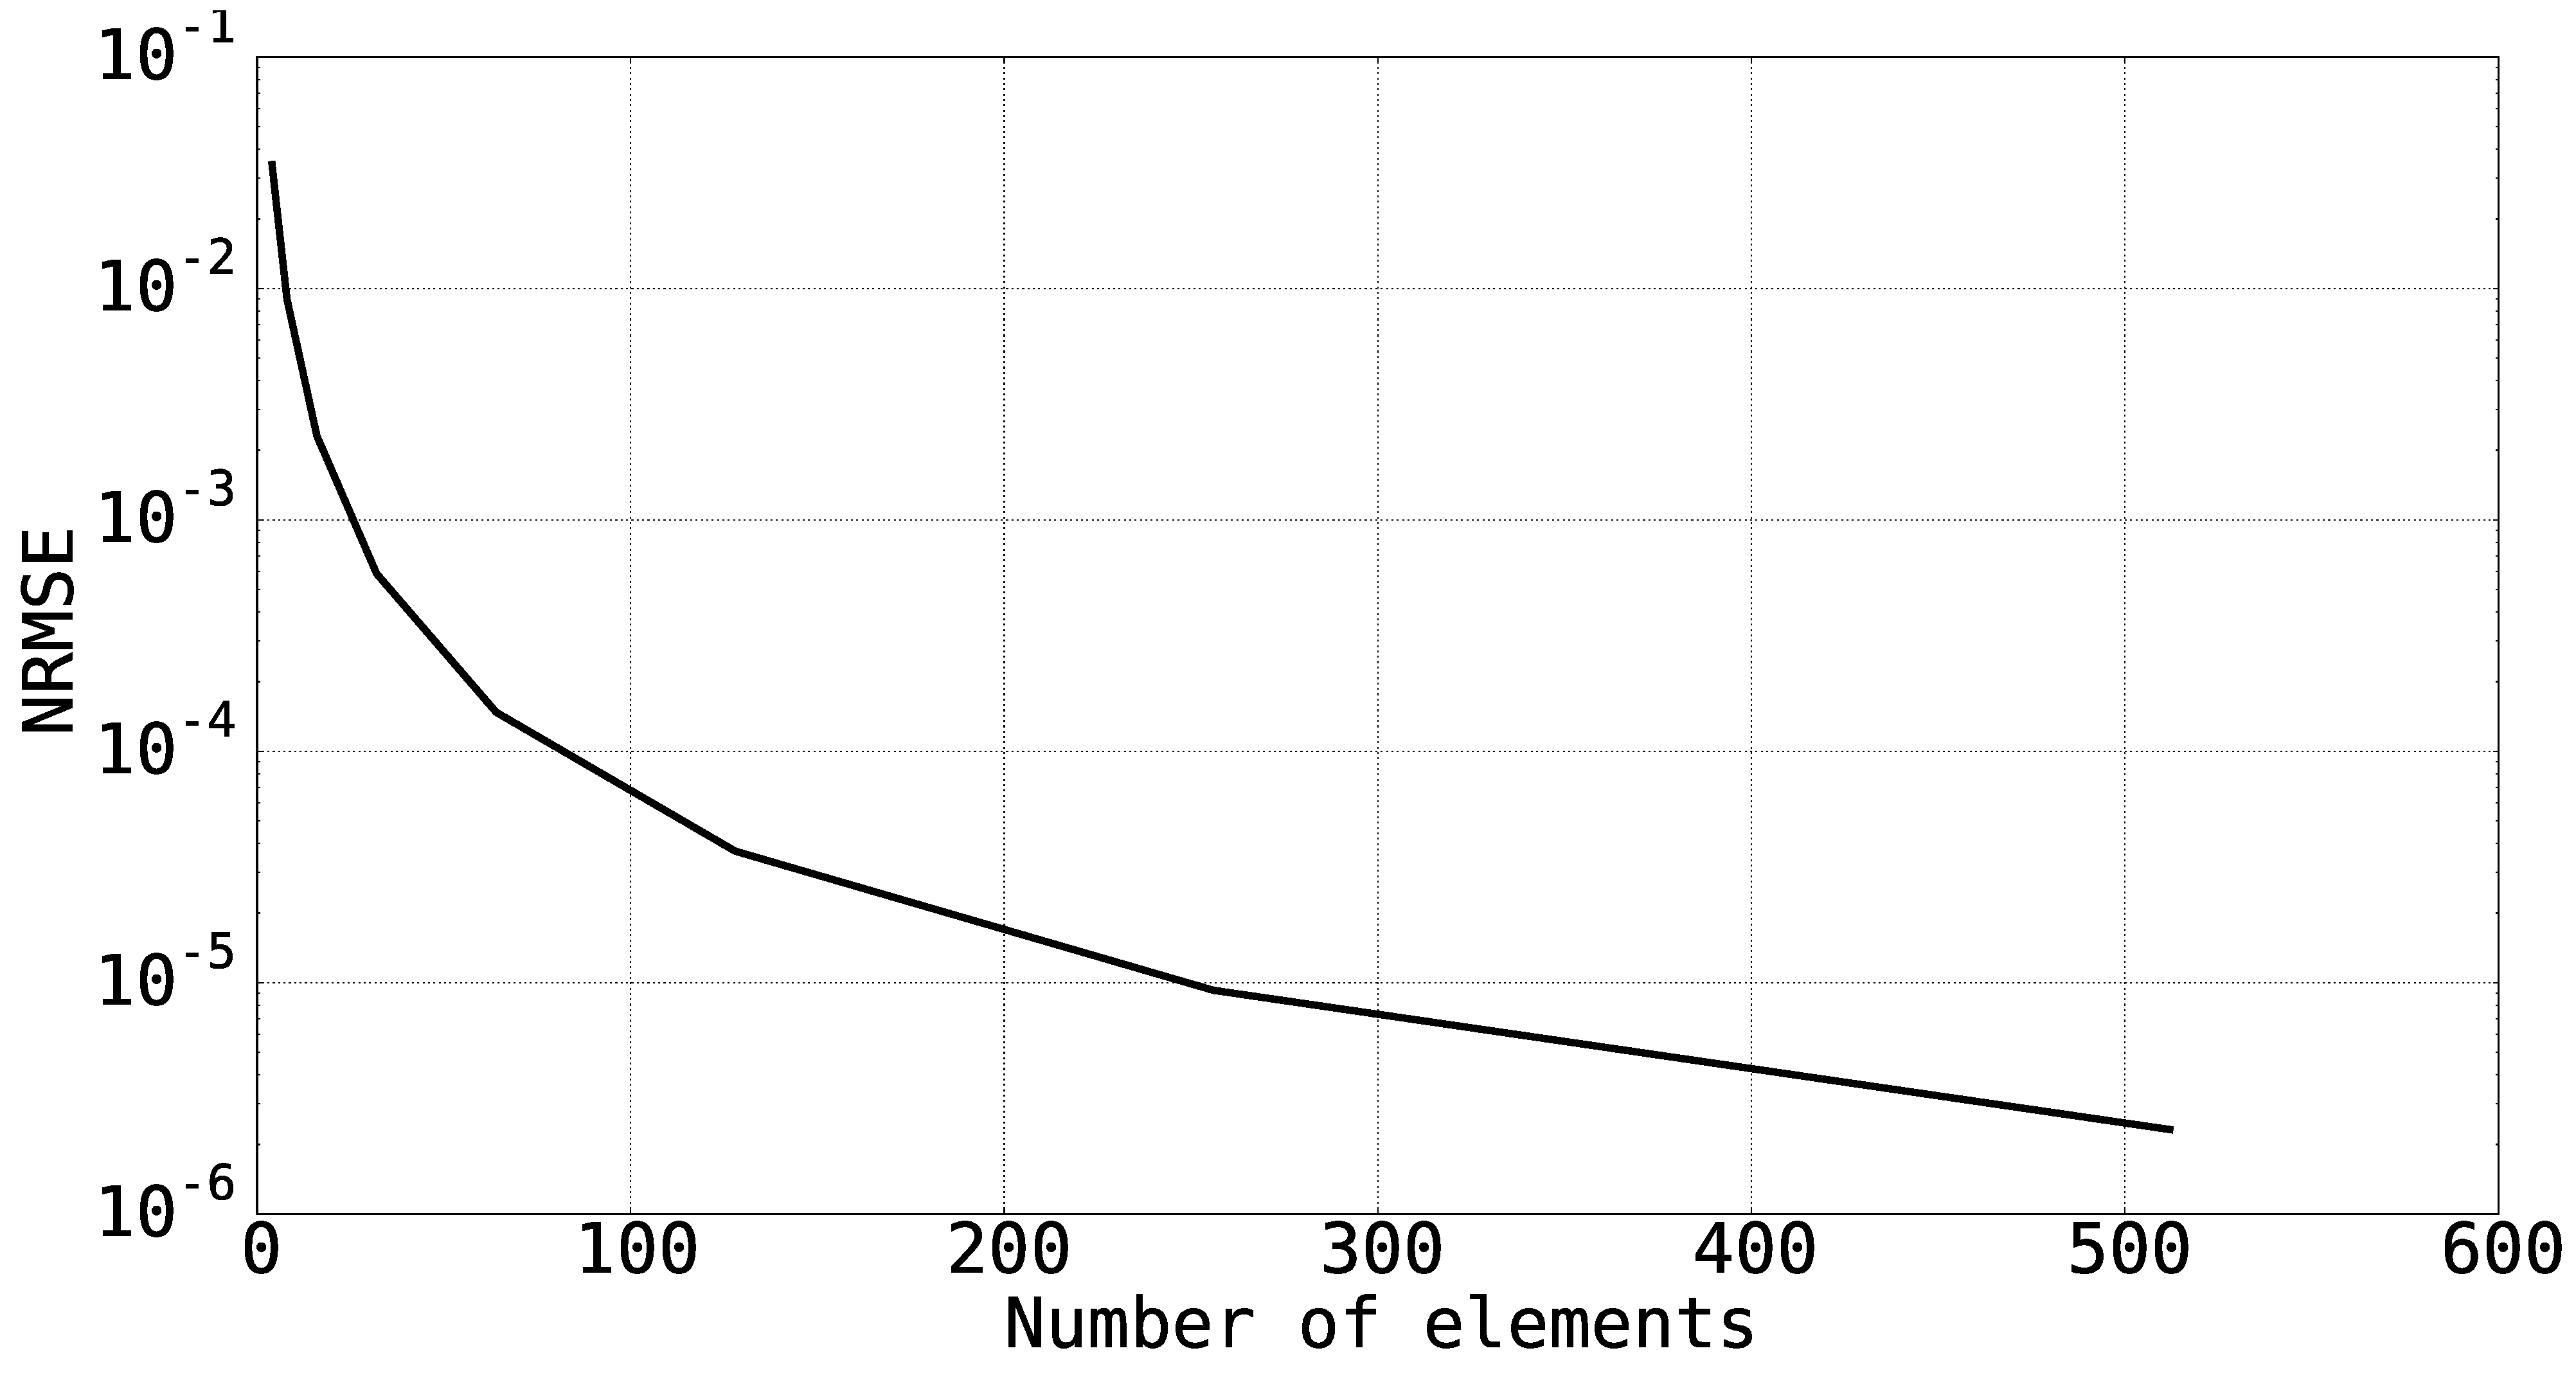
\includegraphics[width=14.00cm]{Chapter_2/figure/axial_bar_governing_equation_mesh_convergence.eps}
	\caption{Mesh convergence of the finite elements analysis for axial bar.}
	\label{fig:C2_axialBarSolution}
\end{figure}

The discrete sensitivity equation is derived by differentiating Equation \eqref{eq:C2_discretizedBarEquation} with respect to the shape of the domain as shown in Equation \eqref{eq:C2_discretizedSAequation_beforeSimplification}.

\begin{equation}\label{eq:C2_discretizedSAequation_beforeSimplification}
	\left[ \frac{\partial K}{\partial b} - \frac{\partial K_s}{\partial b} \right] [U] + 
	[K - K_s] \left[ \frac{\partial U}{\partial b} \right] = 
	\left[ \frac{\partial F_d}{\partial b} \right] - 
	\left[ \frac{\partial F_p}{\partial b} \right]
\end{equation}

where $b$ is the design variable. $[K_s]$ is not affected by the design variable, therefore its derivative with respect to $b$ is equal to zero. Same argument can be made for the point load $F_p$. Using these observations, Equation \eqref{eq:C2_discretizedSAequation_beforeSimplification} is simplified as

\begin{equation}\label{eq:C2_discretizedSensitivityEquation}
	\left[ \frac{\partial U}{\partial b} \right] = 
	[K - K_s]^{-1}
	\left\{
	\left[ \frac{\partial F_d}{\partial b} \right] - \left[ \frac{\partial K}{\partial b} \right] [U]
	\right\}
\end{equation}

In Equation \eqref{eq:C2_discretizedSensitivityEquation}, $[U]$ is known as the result of solving the governing equation \eqref{eq:C2_discretizedBarEquation}, and $\dfrac{\partial F_d}{\partial b}$ is easily calculated since the distributed force is analytically known. $\dfrac{\partial K}{\partial b}$ is calculated by differentiating Equation \eqref{eq:C2_stiffnessMatrixOfBar}. It should be noted that change in the length of the bar, $L$, only affects $l_3$. Therefore, $\dfrac{\partial l_3}{\partial L}$ is equal to one. Finally, the sensitivity of stiffness matrix to the shape design variable for a simple case of Equation \eqref{eq:C2_stiffnessMatrixOfBar} is written as

\begin{equation}\label{eq:C2_sensitivityOfStiffnessMatrixOfBar}
	\left[ \frac{\partial K}{\partial L} \right] = 
	-EA
	\begin{bmatrix}
	0 & 0 & 0 & 0 \\
	0 & 0 & 0 & 0 \\
	0 & 0 & 1/l_3^2 & -1/l_3^2 \\
	0 & 0 & -1/l_3^2 & 1/l_3^2
	\end{bmatrix}
\end{equation}
% ======================================================================================
\section{Continuum Sensitivity Analysis}
% -.-.-.-.-.-.-.-.-.-.-.-.-.-.-.-.-.-.-.-.-.-.-.-.-.-.-.-.-.-.-.-.-.-.-
\subsection{Formulation}
For a continuous system, the governing equations and boundary conditions are written as
%
\begin{subequations}\label{eq:C2_continuumGoverningEquation}
\begin{align}
    A(u, t; b) &= 0 \qquad \qquad \text{on } \Omega \\
    B(u, t; b) &= g(x, t; b) \quad \text{on } \Gamma
\end{align}    
\end{subequations}
%
where $u$ is the response variable, i.e. displacement or pressure, $t$ is time, $x$ is the spatial coordinate, and $b$ is the design variable that can be used to control the solution. $A$ and $B$ are continuum functions that define the governing equations and boundary conditions respectively. It should be noted that the governing equation is written in the residual form where its value needs to be equal to zero when $u$ is the solution at time $t$. $g$ is the value of the boundary condition of the defined system. To calculate the response sensitivity, the total derivative of Equation \eqref{eq:C2_continuumGoverningEquation} is required. This is done by determining the local sensitivity of the governing equation followed by converting the local sensitivities to their total form using Equation \eqref{eq:C2_totalSensitivityDef}.

The governing equation while the boundary condition of \eqref{eq:C2_continuumGoverningEquation} is differentiated as follows
%
\begin{subequations}\label{eq:C2_continuumSensitivityFormulation}
\begin{align}
    A(u', t; b) + A'(u, t; b) &= 0 \qquad \qquad \text{on } \Omega \\
    B(\dot{u}, t; b) + \dot{B}(u, t; b) &= \dot{g}(x, t; b) \quad \text{on } \Gamma
\end{align}    
\end{subequations}
%
where $(\text{ })'$ and $\dot{(\text{ })}$ are local and total derivative which are defined as follows
%
\begin{subequations}
\begin{align*}
    (\text{ })' &= \frac{\partial (\text{ })}{\partial b} \\
    \dot{(\text{ })} &= \frac{D (\text{ })}{D b}
\end{align*}
\end{subequations}
%
It should be noted that the governing equations are differentiated in the local form, and the boundary conditions are differentiated in the total form. Local differentiation of the governing equations enables us to treat the solver non-intrusively \cite{cross2014local}. However, to capture the effect of shape change, the boundary conditions need to be differentiated in the total form. The boundary condition definition is further simplified by assuming the $\mathbf{B}$ operator is linear and remains the same throughout the analysis. This is a valid assumption for many practical cases such as structural analysis or computational fluid dynamics. The boundary conditions are typically in the form of known gradient or values, i.e. outflow and free-slip wall for CFD and predefined displacement/force for structural analysis. It should be noted that this assumption is not valid for problems such as contacts. The boundary condition is written as:
%
\begin{align}\label{eq:C2_linearSAboundaryCondtions}
\begin{split}
    B(\dot{u}, t; b) &= \dot{g}(x, t; b) \Rightarrow \\
    B(u', t; b) &= \dot{g}(x, t; b) - B(\frac{\partial u}{\partial x} \cdot \frac{\partial x}{\partial b}, t; b)
\end{split}
\end{align}
%
To study the differentiated governing equation of Equation \eqref{eq:C2_continuumSensitivityFormulation}, we will assume two situations: i) linear analysis and ii) nonlinear analysis.

For the linear analysis, the governing  of \eqref{eq:C2_continuumSensitivityFormulation} is written as:
%
\begin{equation}\label{eq:C2_linearSAgoverningEquation}
    A(u', t; b) = 0 
\end{equation}
%
This is valid for the linear case because the differential operators of the governing equation do not depend on the response variable, $u$. To explain this concept we look at the transient heat conduction in the 1D domain. The governing equations are defined as
%
\begin{equation}\label{eq:C2_transientHeatCondtionGE}
    \frac{\partial^2 T}{\partial x^2} = \frac{1}{\alpha} \frac{\partial T}{\partial t}
\end{equation}
%
where $T$ is the temperature, $x$ is spatial coordinate, $t$ is time, and $\alpha$ is is the thermal diffusivity ($k/\rho c_p$). This equation can be differentiated with respect to a design variable $b$ as shown in the following equation.
%
\begin{equation*}
    \frac{\partial}{\partial b}
    \left( \frac{\partial^2 T}{\partial x^2}\right) = 
    \frac{\partial}{\partial b}
    \left( \frac{1}{\alpha} \frac{\partial T}{\partial t}\right)
\end{equation*}
%
Due to linearity of the differential operators we can change the order of differentiation as follows:
%
\begin{equation}\label{eq:C2_transientHeatCondtionSA}
    \frac{\partial^2}{\partial x^2}
    \left( \frac{\partial T}{\partial b} \right) = 
    \frac{1}{\alpha} \frac{\partial}{\partial t}
    \left( \frac{\partial T}{\partial b}\right)
\end{equation}
%
By comparing Equations \eqref{eq:C2_transientHeatCondtionGE} and \eqref{eq:C2_transientHeatCondtionSA} we can see that the differential operators $\partial^2 /\partial x^2$ and $\partial /\partial t$ remain unchanged. Therefore the same solver can be used for solving this system of governing equations and for the sensitivity variable, $\partial T/\partial b$.

For nonlinear problems, the differential operators are functions of response variables as well. For example, the incompressible Euler's equation for a 2D flow is derived as
%
\begin{subequations}\label{eq:C2_eulerEquations}
\begin{gather}
    \frac{\partial u}{\partial t} +
    u \frac{\partial u}{\partial x} + v \frac{\partial u}{\partial y} +
    \frac{\partial p}{\partial x} = 0 
    \\
    \frac{\partial v}{\partial t} +
    u \frac{\partial v}{\partial x} + v \frac{\partial v}{\partial y} +
    \frac{\partial p}{\partial y} = 0
\end{gather}
\end{subequations}
%
where $u$ and $v$ are the velocity components in $x$ and $y$ directions respectively. $p$ is pressure, $t$ is time, and $x$ and $y$ are spatial coordinates. We can rewrite Equation \eqref{eq:C2_eulerEquations} in terms of differential operators as well.
%
\begin{subequations}
\begin{gather*}
    \mathcal{T} u +
    \mathcal{C} u +
    \mathcal{G}_x p = 0 
    \\
    \mathcal{T} v +
    \mathcal{C} v +
    \mathcal{G}_y p = 0 
\end{gather*}
\end{subequations}
%
where $\mathcal{T}$ is the time derivative operator ($\partial /\partial t$) and $\mathcal{C}$ is the convective operator
%
\begin{equation}\label{eq:C2_convectiveOperator}
    \mathcal{C} = u \frac{\partial}{\partial x} + v \frac{\partial}{\partial y}
\end{equation}
%
and $\mathcal{G}_x$ and $\mathcal{G}_y$ are gradient operators in $x$ and $y$ respectively ($\partial /\partial x$ and $\partial /\partial y$). The gradient and time derivative operators are linear; therefore, they can be treated as shown in the previous paragraphs. On the other hand, the convective operator is nonlinear and should be differentiated with response variables as well. As a result, the sensitivity equations can be written in the operator form as
%
\begin{subequations}\label{eq:C2_eulerEquationsSA}
\begin{gather}
    \mathcal{T} u' +
    \mathcal{C}' u + \mathcal{C} u' +
    \mathcal{G}_x p' = 0 
    \\
    \mathcal{T} v' +
    \mathcal{C}' v + \mathcal{C} v' +
    \mathcal{G}_y p' = 0 
\end{gather}
\end{subequations}
%
where
%
\begin{equation*}
    \mathcal{C}' = u' \frac{\partial}{\partial x} + v' \frac{\partial}{\partial y}
\end{equation*}
%
Several interesting properties of CSA can be explained using Equation \eqref{eq:C2_eulerEquationsSA}. Importantly, although the original Euler equation is nonlinear due to the multiplication of response variables and their derivatives ($u$ and $\partial u/\partial x$), the resulting sensitivity equation is linear. This means that the sensitivity equations are easier to solve both concerning algorithms and simulation time compared to the original equations. The challenging expression that needs to be calculated in Equation \eqref{eq:C2_eulerEquationsSA} is the convective term derivative.

The first step in solving the sensitivity equations is to find the solution of the governing equations. This enables us to calculate the convective operator, $\mathcal{C}$, at each step of sensitivity solution based on the analysis data. $\mathcal{C}'$ is also calculated at each step of the solution of sensitivity equations based on the solution of the previous time step. For a simple predictor-corrector method used to solving the original governing equations, this can be written as follows for sensitivity equation in $x$ direction.
%
\begin{align*}
    \bar{u}' &= u'(i) - 
    \Delta t \left[ \mathcal{C}'(i) u(i) + \mathcal{C}(i) u'(i) + \mathcal{G} p'(i) \right]
    \qquad \text{: predictor}
    \\
    u'(i+1) &= u'(i) + \frac{\Delta t}{2} - 
    \left[ \mathcal{C}'(i) u(i) + \mathcal{C}(i) u'(i) + \right. \\
    &\quad \left.  \mathcal{G} p'(i) + \bar{\mathcal{C}}(i) u(i) + \mathcal{C}(i) \bar{u} + \mathcal{G} p'(i)\right]
    \qquad \qquad \quad \text{: corrector}
\end{align*}
%
Here, $\bar{\mathcal{C}}$ in the convective operator is evaluated using $\bar{u}$. It should be noted that to generate the operator we do not need to know the details of how it has been put together. We only supply the required values of the state variables for generating the convective operator; the black-box solver will generate it for us. This input is the response variable when solving the governing equation and is the sensitivity of response variable for sensitivity analysis. Therefore, the solver can still be considered as a black box that we do not modify.
% -.-.-.-.-.-.-.-.-.-.-.-.-.-.-.-.-.-.-.-.-.-.-.-.-.-.-.-.-.-.-.-.-.-.-.-.-.-.-.-.-.-.-.-.-.-
\subsection{Implementation on heat transfer problem}
In this section, the continuum sensitivity formulation is used for calculating the sensitivity of temperature with respect to the length of a 1D domain. The domain is defined in Figure \ref{fig:C2_benchmarkCase} with the temperature in the domain governed by Equation \eqref{eq:C2_laplaceEquation}. The boundary conditions are defined as $T_0$ at $x=0$ and $T_L$ at $x=L$.

To get the sensitivity equations, governing equations are differentiated in the local form and boundary conditions are differentiated in total form as shown in Equation \eqref{eq:C2_differentiatedLaplaceEquation}.
%
\begin{equation}\label{eq:C2_differentiatedLaplaceEquation}
    \frac{\partial}{\partial L}
    \left( \frac{\partial^2 T}{\partial x^2} = 0 \right)
\end{equation}
%
Since the differential operator is linear, the order of differentiations is changed. This will give us the Equation \eqref{eq:C2_laplaceSAequation} for the sensitivity calculation.
%
\begin{equation}\label{eq:C2_laplaceSAequation}
    \frac{\partial^2}{\partial x^2} \left( \frac{\partial T}{\partial L} \right) = 0
\end{equation}
%
The boundary conditions for this problem are written as follows to be consistent with the general formulation of the boundary conditions. 
%
\begin{equation}\label{eq:C2_laplaceEquationBoundaryCondition}
\begin{cases}
    \mathcal{B}T = T_0 \qquad \text{at x = 0} \\
    \mathcal{B}T = T_L \qquad \text{at x = L}
\end{cases}
\end{equation}
%
Where $\mathcal{B}$ is the operator acting on the boundary. For this problem, it is equal to $1$. Equation \eqref{eq:C2_laplaceEquationBoundaryCondition} is differentiated in the total form, since the boundaries are moving. This results in
%
\begin{equation}
\begin{cases}
    \dot{\mathcal{B}} T + \mathcal{B} \dot{T} = \dot{T}_0 \qquad \text{at x = 0} \\
    \dot{\mathcal{B}} T + \mathcal{B} \dot{T} = \dot{T}_L \qquad \text{at x = L}
\end{cases}
\end{equation}
%
where $\mathcal{B}$ and $\dot{T}_0$ are constants and have zero derivatives. $\dot{T}$ is written in terms of the local derivative and convective terms using the chain rule. This results in the following definition for the sensitivity equation boundary conditions.
%
\begin{equation*}
\begin{cases}
    \dfrac{\partial T}{\partial b} = -\dfrac{\partial T}{\partial x} \dfrac{\partial x}{\partial b} \qquad \text{at x = 0}
    \\
    \dfrac{\partial T}{\partial b} = -\dfrac{\partial T}{\partial x} \dfrac{\partial x}{\partial b} \qquad \text{at x = L}
\end{cases}
\end{equation*}
%
To calculate the mesh sensitivity at the boundary, the dependency of the spatial variable, $x$, and the shape of the domain, $L$, need to be known. For the 1D domain, this is defined as follows:
%
\begin{equation*}
    x = \alpha L
\end{equation*}
%
This means that every location in the domain can be defined using a nondimensional variable, $\alpha$, times the total length of the domain. Using this formulation, the sensitivity of spatial coordinate, $x$, with respect to the length of the domain is defined as:
%
\begin{equation*}
    \frac{\partial x}{\partial L} = \alpha \quad \text{where } \quad \alpha = \frac{x}{L}
\end{equation*}
%
By using this relation, the boundary conditions can be written as:
%
\begin{equation*}
\begin{cases}
    \mathcal{B} \dfrac{\partial T}{\partial b} = -\dfrac{\partial T}{\partial x} \dfrac{x}{L} \qquad \text{at x = 0}
    \\
    \mathcal{B} \dfrac{\partial T}{\partial b} = -\dfrac{\partial T}{\partial x} \dfrac{x}{L} \qquad \text{at x = L}
\end{cases}
\end{equation*}
%
This can be further simplified by substituting $x$ in the definition of boundary conditions. We also substitute $\mathcal{B}$ as 1.
%
\begin{equation}\label{eq:C2_laplaceSAboundaryCondition}
\begin{cases}
    \dfrac{\partial T}{\partial b} = 0 \qquad \text{at x = 0}
    \\
    \dfrac{\partial T}{\partial b} = -\dfrac{\partial T}{\partial x} \qquad \text{at x = L}
\end{cases}
\end{equation}
%
The last thing to be noted is the spatial derivative of response variable at the boundaries, $\partial T/\partial x$. This term appears due to the boundary movement with a change in shape design variable when using the chain rule. This term is calculated from the analysis results by using the same technique used for discretizing the governing equations. For this problem, the finite difference method is used to calculate this derivative from the analysis results.

The governing equation of \eqref{eq:C2_laplaceSAequation} with boundary condition \eqref{eq:C2_laplaceSAboundaryCondition} is solved using the same solver that we used for solving the original governing equation since these two are effectively having the same form. The comparison between the original governing equation and the sensitivity equation is shown in Table \ref{table:C2_comparisonBetweenGEandSA}.
%
\begin{table}[h]
\begin{tabular}{| c | c | c | c | c |}
    \hline
    Analysis Type & Equation & Unknown & Discretized form & Discretization \\ \hline \hline
    Governing equation & $\partial^2 T/\partial x^2$ & $T$ & $[K][T] = [F_{BC}]$ & Central difference \\ \hline
    Sensitivity equation & $\partial^2 T'/\partial x^2$ & $T'$ & $[K][T'] = [F'_{BC}]$ & Central difference \\ \hline
\end{tabular}
\caption{Comparison between the governing and sensitivity equations.}
\label{table:C2_comparisonBetweenGEandSA}
\end{table}
%
The continuum sensitivity analysis (CSA) result is verified using the analytical solution of Equation \eqref{eq:C2_benchmarkCaseAnalyticalSolution} as shown in Figure \ref{fig:C2_comparisonBetweenCSAandAnalytical}. Different number of discretization nodes are used for the comparison between the results. For the qualitative comparison between the results, the NRMSD as defined in Equation \eqref{eq:C2_NRMSD} is used. As shown if Figure \ref{fig:C2_comparisonBetweenCSAandAnalytical} and Table \ref{table:C2_CSA_NRMSD}, the two results match perfectly.
%
\begin{figure}[H]
    \centering
    \subfigure[$n = 11$]
    {
    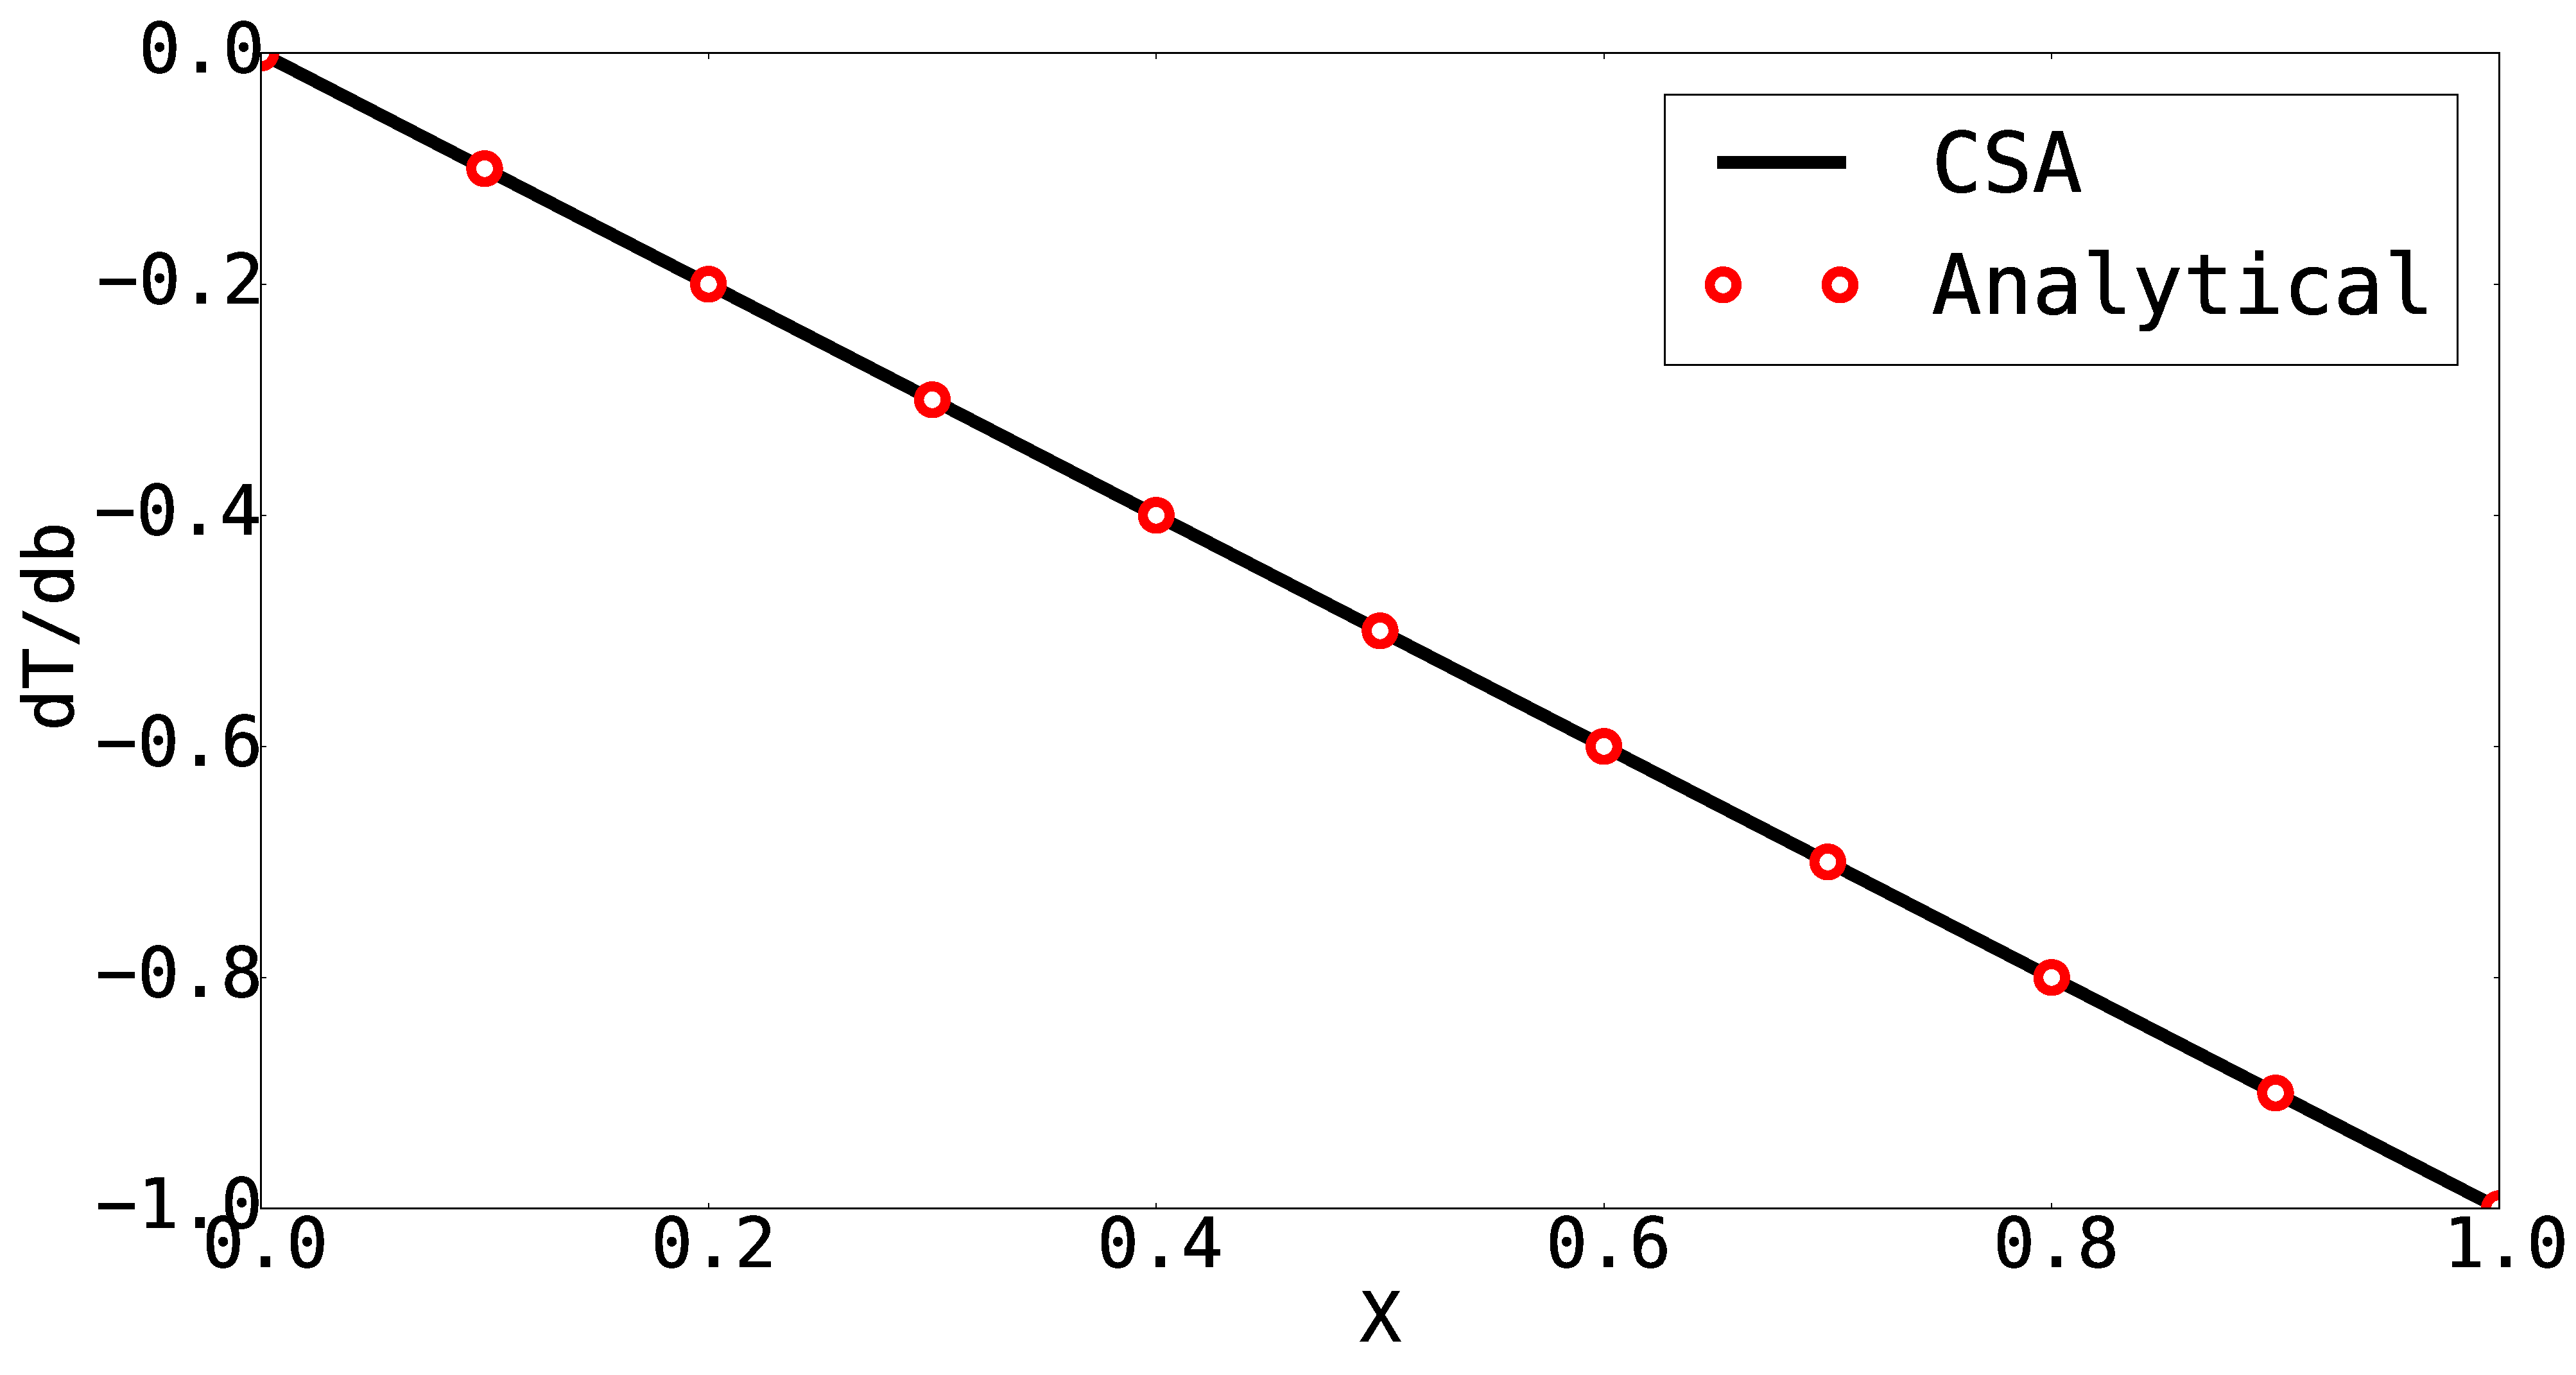
\includegraphics[width=6.5cm]{Chapter_2/figure/CSA_n11.eps}
    }
    \quad
    \subfigure[$n = 41$]
    {
    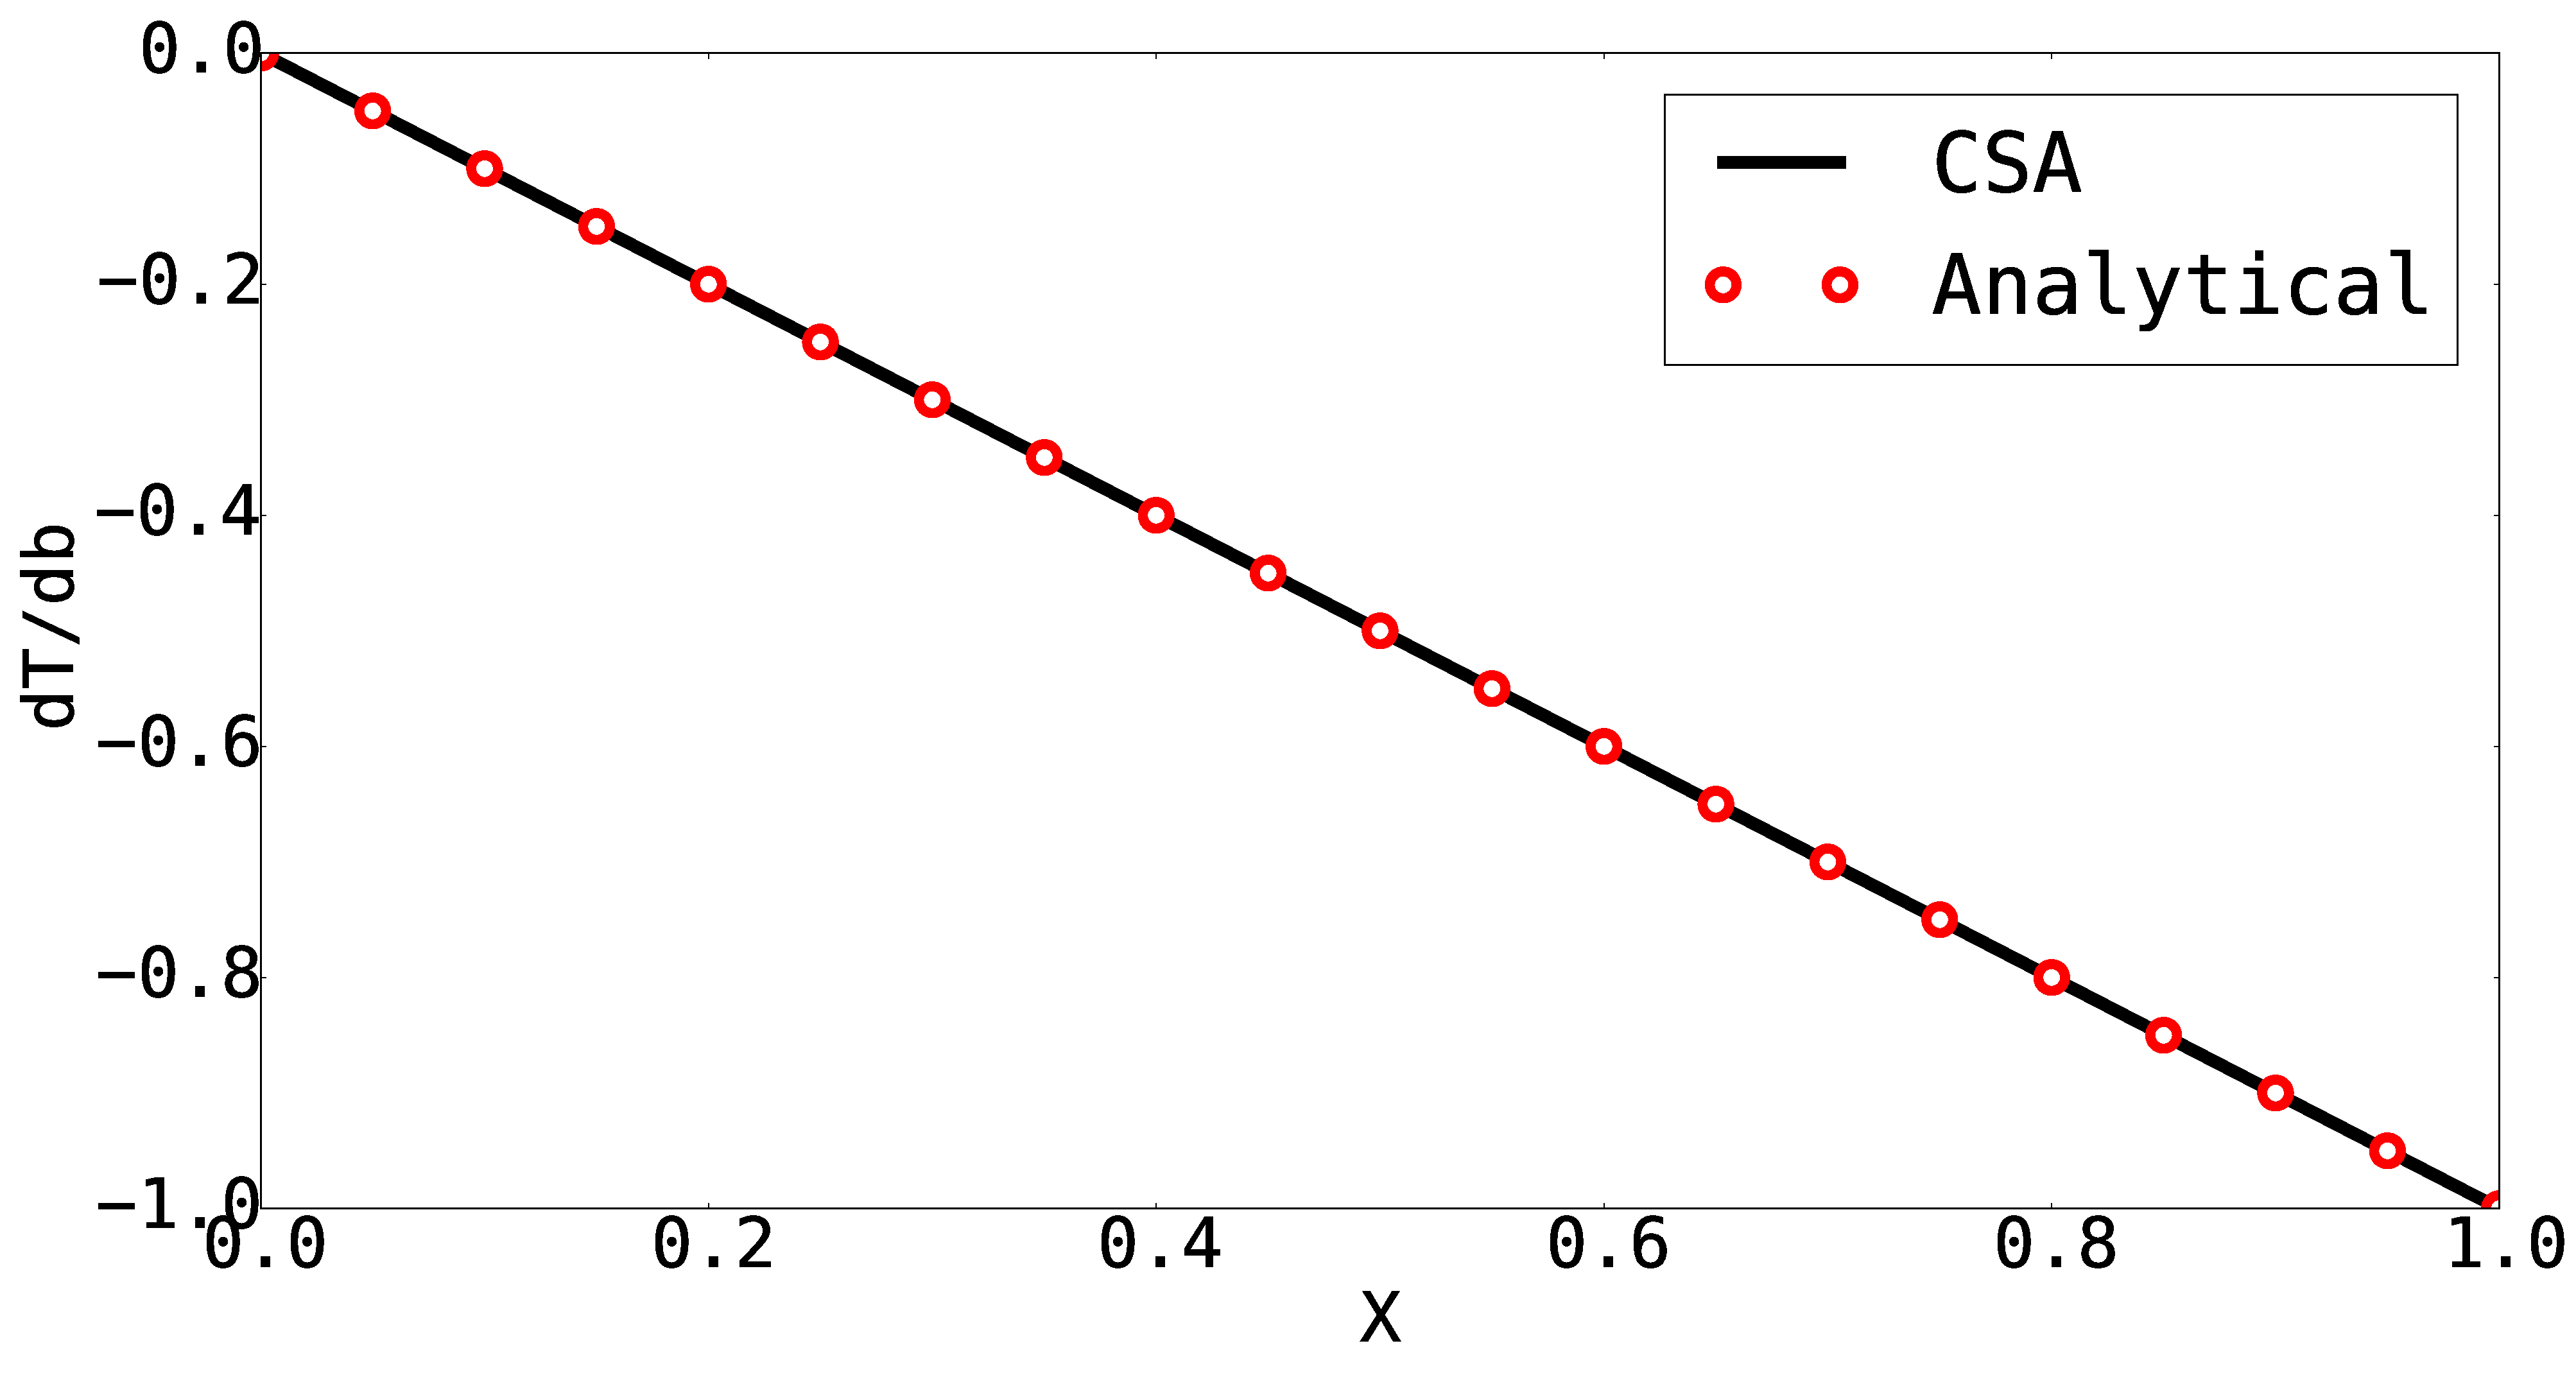
\includegraphics[width=6.5cm]{Chapter_2/figure/CSA_n41.eps}
    }
    \\
    \subfigure[$n = 81$]
    {
    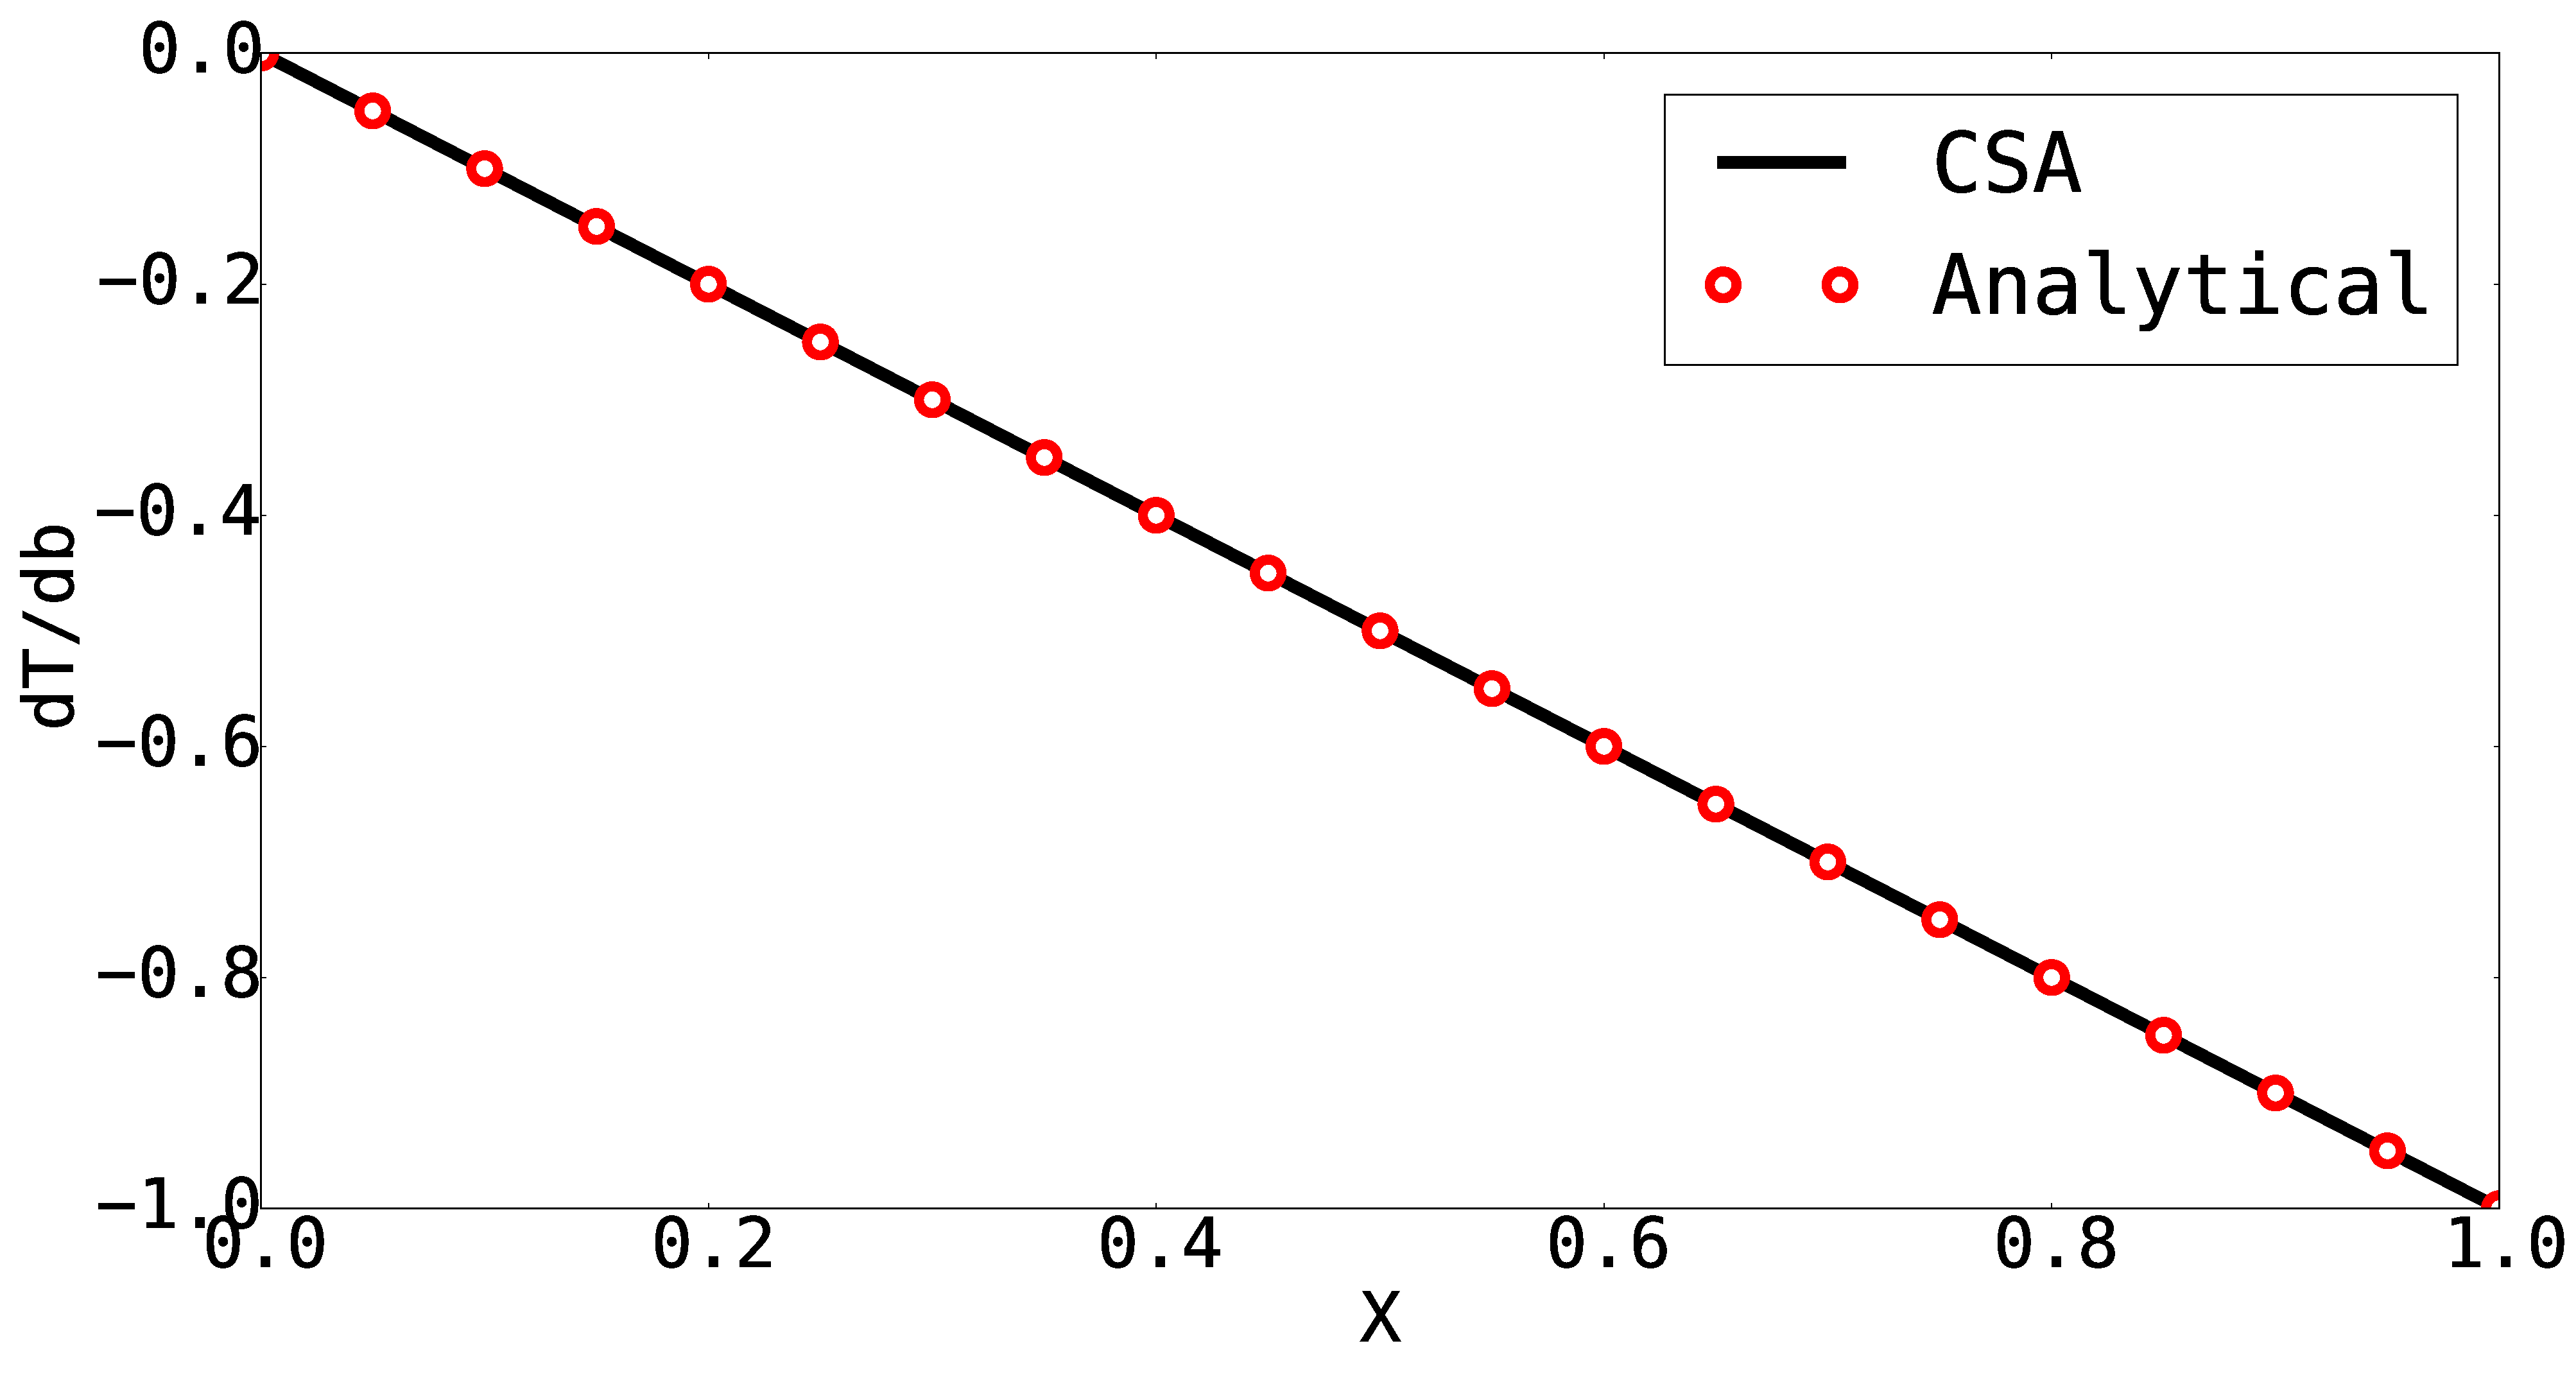
\includegraphics[width=6.5cm]{Chapter_2/figure/CSA_n81.eps}
    }
    \quad
    \subfigure[$n = 161$]
    {
    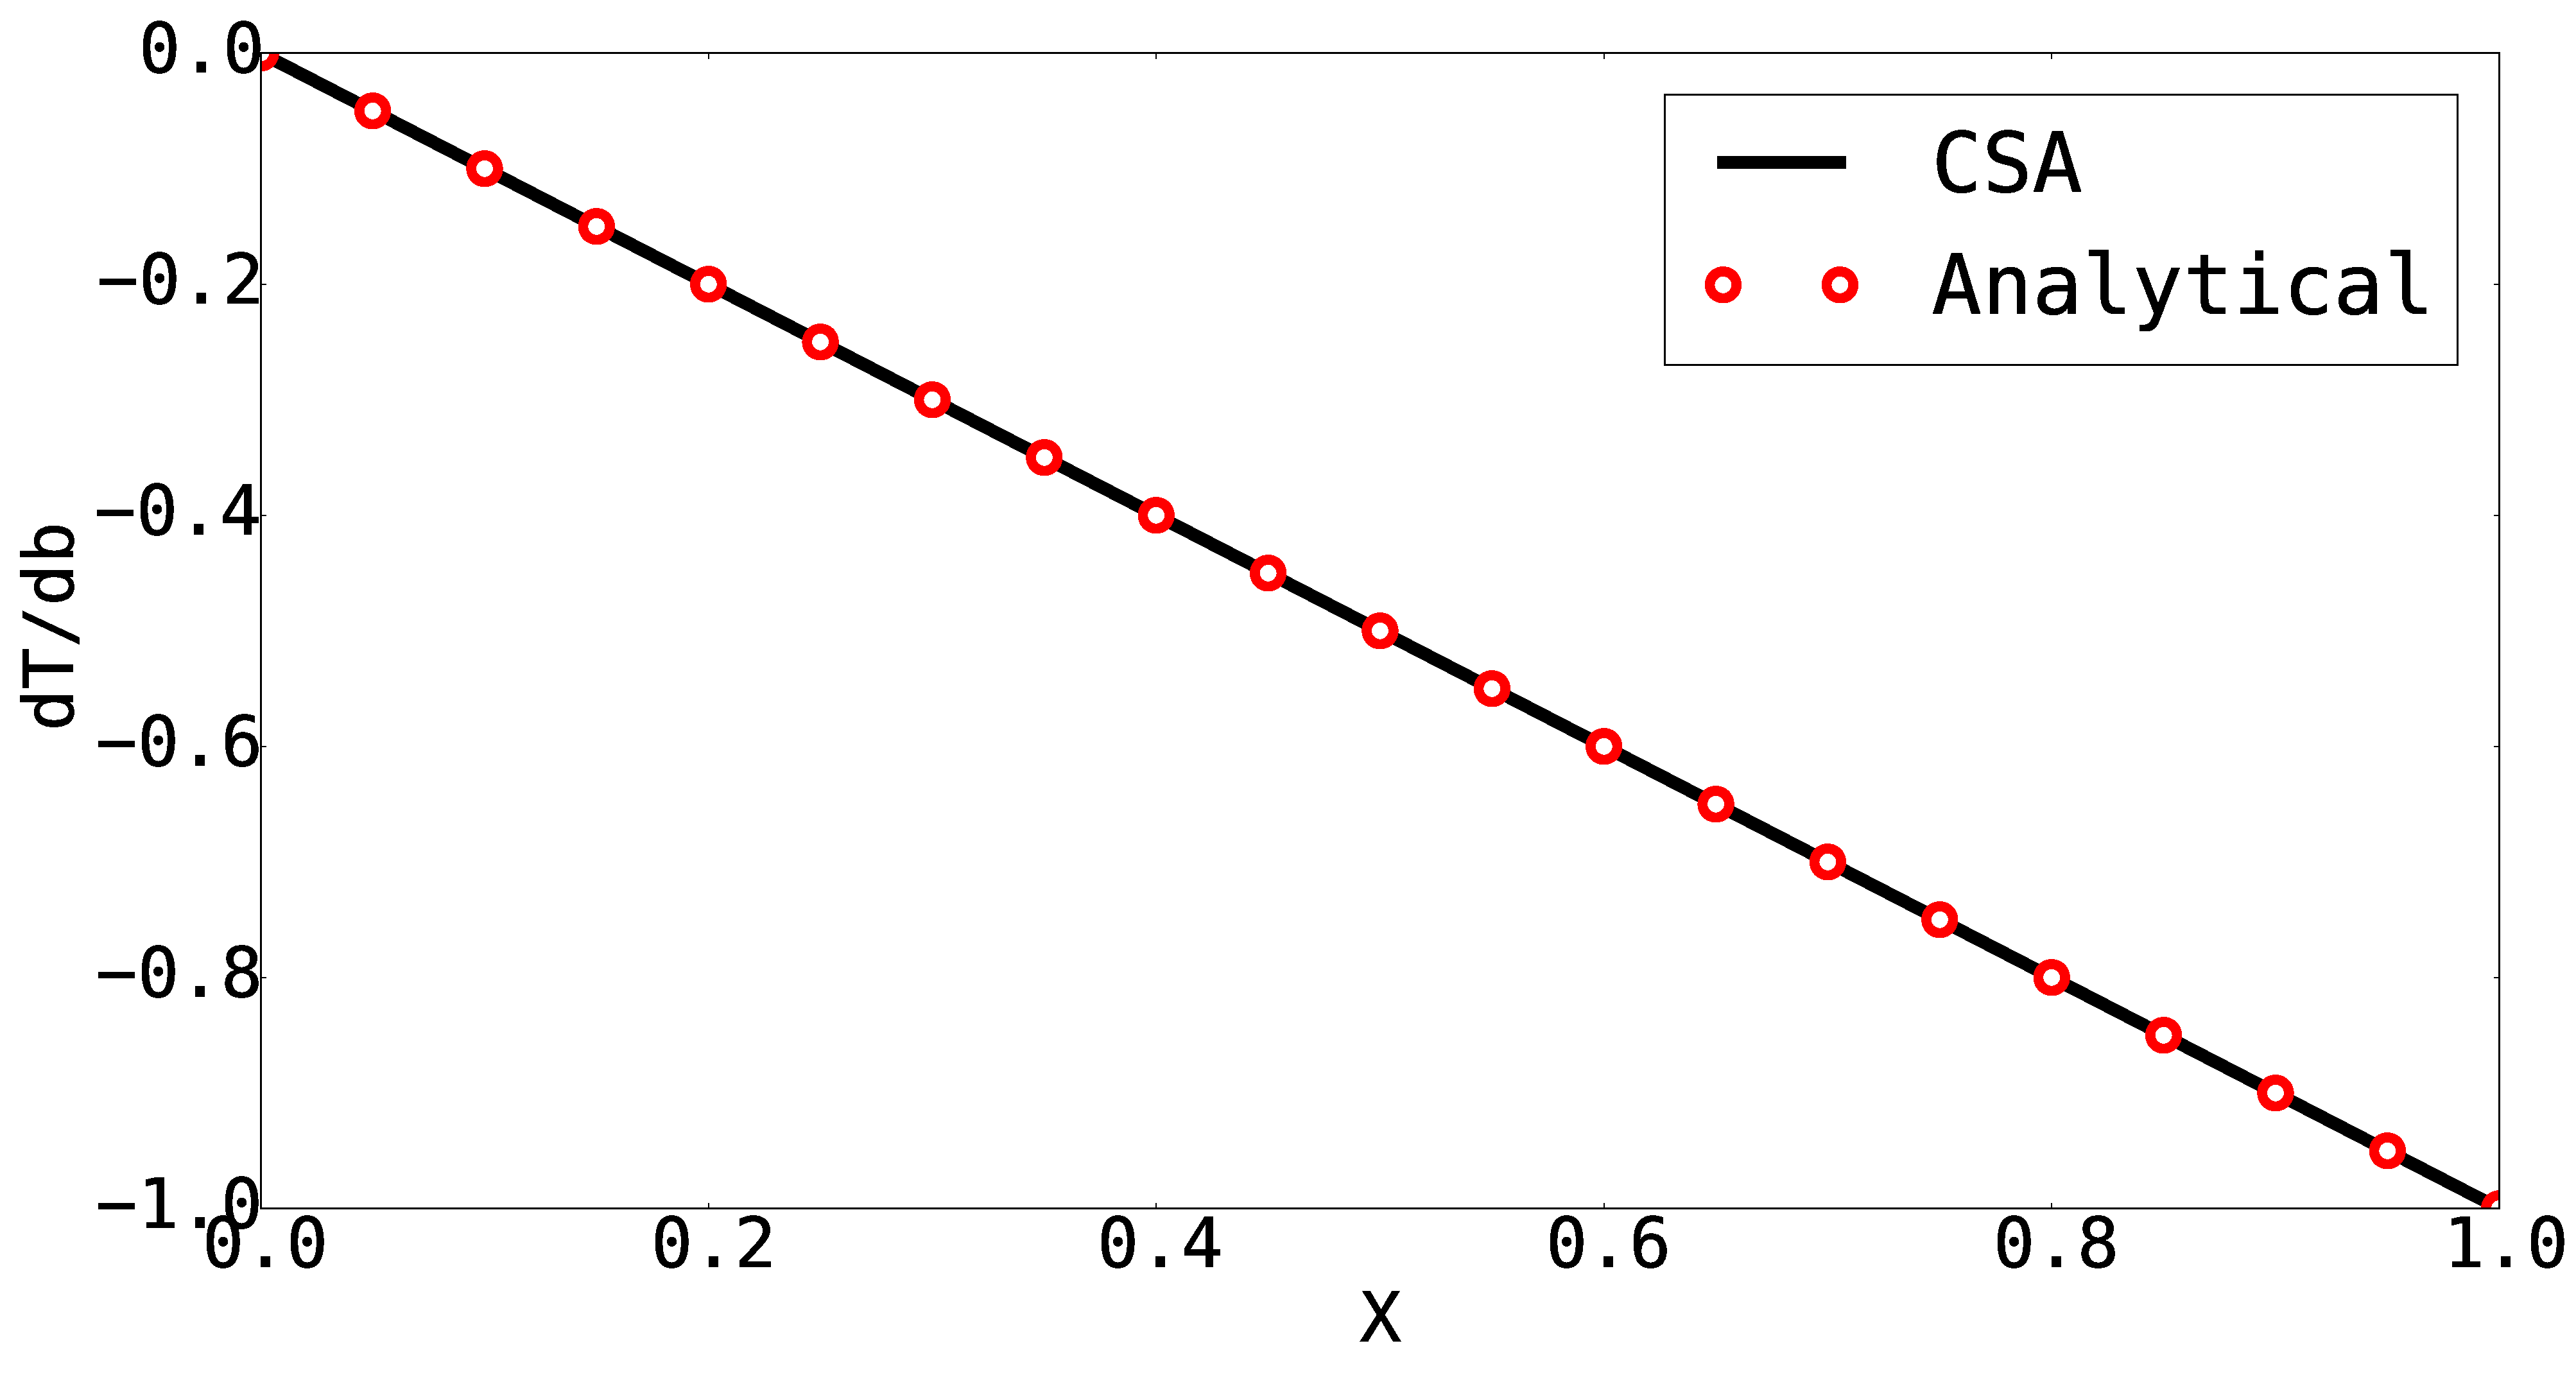
\includegraphics[width=6.5cm]{Chapter_2/figure/CSA_n161.eps}
    }
    \caption{Comparison between continuum sensitivity analysis and analytical results for different number of nodes.}
    \label{fig:C2_comparisonBetweenCSAandAnalytical}
\end{figure}
%
%
\begin{table}[H]
\centering
\begin{tabular}{| c | c |}
    \hline
    Number of nodes & NRMSD \\ \hline \hline
    11 & $6.96 \times 10^{-17}$ \\ \hline
    41 & $2.02 \times 10^{-15}$ \\ \hline
    81 & $1.43 \times 10^{-15}$ \\ \hline
    161 & $2.77 \times 10^{-15}$ \\ \hline
\end{tabular}
\caption{RMSE value for different number of nodes.}
\label{table:C2_CSA_NRMSD}
\end{table}
%
It should be noted that the sensitivity equations are derived and solved in the local form. This does not include the effect of nodes moving in the computational domain. If the analysis requires the sensitivity at the material points, an additional step is required to convert the local sensitivities to their total form using the chain rule as shown in the following equation.
%
\begin{equation*}
    \frac{DT}{Db} = \frac{\partial T}{\partial b} + \frac{\partial T}{\partial x} \cdot \frac{\partial x}{\partial b}
\end{equation*}
%
This will add an extra cost to the simulation due to the additional step for calculating $\partial x/\partial b$. The reason this step exists is due to movement of computational nodes as the results of a change in shape. Therefore, if the computational nodes can be fixed, the $\partial x/\partial b$ term will be equal to zero. We are proposing to achieve this using a non-body conformal technique such as immersed boundary method. This will be explained in the next chapter in more detail.
% -.-.-.-.-.-.-.-.-.-.-.-.-.-.-.-.-.-.-.-.-.-.-.-.-.-.-.-.-.-.-.-.-.-.-.-.-.-.-.-.-.-.-.-.-
\subsection{Implementation on solid mechanics problem}
To derive the continuum sensitivity equations, the governing equation of \eqref{eq:C2_axialBarGE} is differentiated with respect to the design variable, $L$, as shown in Equation \eqref{eq:C2_axialBarContinuumSensitivityEquation}.
%
\begin{equation}\label{eq:C2_axialBarContinuumSensitivityEquation}
    \frac{\partial^2}{\partial x^2} \left( \frac{\partial u}{\partial L} \right) - 
    \frac{\pi x}{L^2} \cos \left( \frac{\pi x}{L} \right) = 0
\end{equation}
%
The boundary conditions are calculated by differentiating the boundary conditions defined in Equation \eqref{eq:C2_axialBarBC}. It should be noted that the boundary conditions are differentiated in total form.
%
\begin{equation}\label{eq:C2_axialBarContinuumSensitivityBoundaryConditions}
    \begin{cases}
    \dfrac{\partial}{\partial x} \left( \dfrac{\partial u}{\partial L} \right) \bigg|_{x = 0} = 
    \dfrac{\partial }{\partial L} \left( \dfrac{1}{\pi} \right) = 0
    \\
    \dfrac{\partial}{\partial x} \left( \dfrac{\partial u}{\partial L} \right) \bigg|_{x = L} = 
    \left\{
    K \left[ \dfrac{\partial u}{\partial L} + \dfrac{\partial u}{\partial x} \dfrac{\partial x}{\partial L} \right] - 
    \dfrac{\partial^2 u}{\partial x^2} \dfrac{\partial x}{\partial L}
    \right\} \bigg|_{x = L}
    \end{cases}
\end{equation}
%
For this problem, the spatial coordinate $x$ is defined as $x = \zeta L$ where $\zeta = x / L$. Therefore, the design velocity $\partial x/\partial L$ at $x = L$ is equal to one. Solving the governing equation \eqref{eq:C2_axialBarContinuumSensitivityEquation} along with boundary conditions \eqref{eq:C2_axialBarContinuumSensitivityBoundaryConditions} leads to the sensitivity values of displacement in the domain, $\partial u/\partial L$. Comparing the sensitivity equation and boundary conditions \eqref{eq:C2_axialBarContinuumSensitivityEquation} and \eqref{eq:C2_axialBarContinuumSensitivityBoundaryConditions} to the governing equation and its corresponding boundary conditions of \eqref{eq:C2_axialBarGE} and \eqref{eq:C2_axialBarBC}, it is safe to say that these equations are the same. The only difference is their boundary conditions. Therefore, the same numerical solver that was used for solving the governing equation can be used to solve the sensitivity equations without any modifications. The only change would be in the values of the boundary conditions. However, change in the boundary conditions does not alter the structure of the black box solver.

To calculate the sensitivities, the governing equation and boundary conditions of \eqref{eq:C2_axialBarContinuumSensitivityEquation} and \eqref{eq:C2_axialBarContinuumSensitivityBoundaryConditions} are discretized using the finite element method as discussed through equations \eqref{eq:C2_stiffnessMatrixOfBar} and \eqref{eq:C2_discretizedBarEquation}. It should be noted that $[K]$ and $[K_s]$ are the same matrices that used in Equation \eqref{eq:C2_stiffnessMatrixOfBar}, $[F_p]$ is equal to zero, and $F_d = -\dfrac{\pi x}{L^2} \cos \left( \dfrac{\pi x}{L} \right)$. For verification, the results for the sensitivity analysis are compared with the analytical results of sensitivity as defined by Equation \eqref{eq:C2_axialBarSensitivitySolution}. We used the NRMSE metric to compare the two different results as defined in Equation \eqref{eq:C2_NRMSE_beam}. The comparison of the results are shown in Figure \ref{fig:C2_continuumSensitivityResults}. As shown here, the results for both discrete and continuum sensitivity analysis converge with the same rate.
%
\begin{figure}[h]
    \centering
    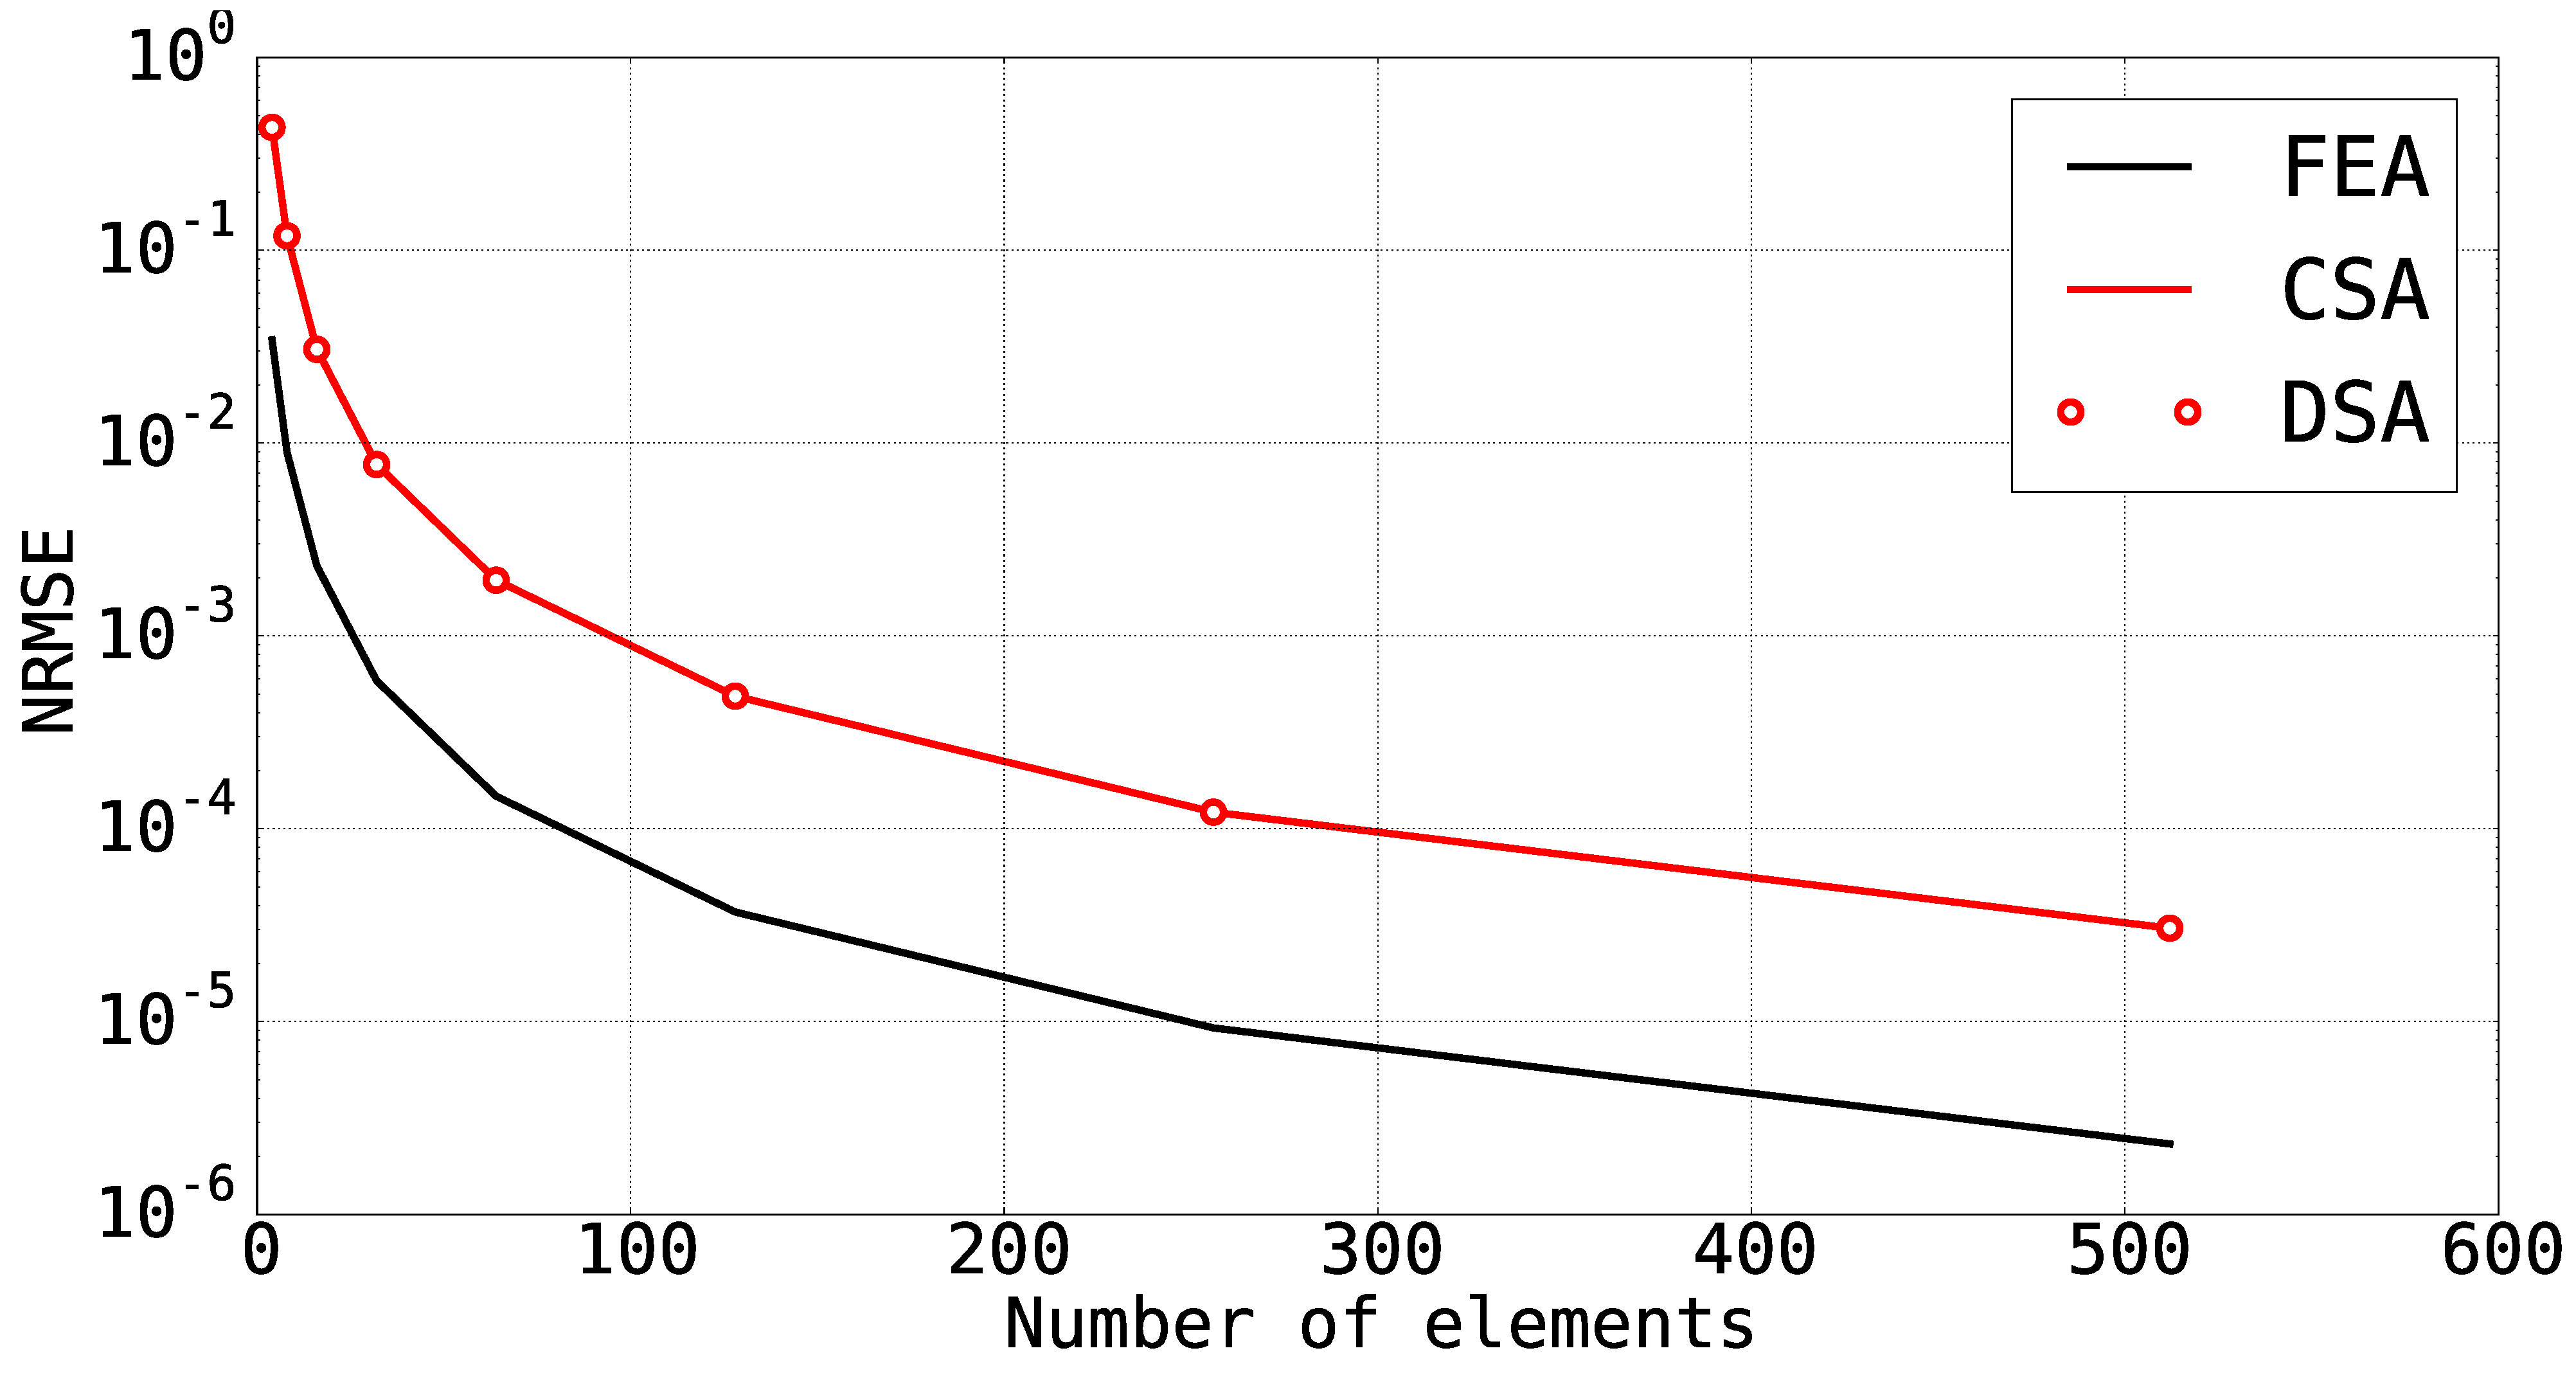
\includegraphics[width=14.00cm]{Chapter_2/figure/axial_bar_continuum_sensitivity_analysis.eps}
    \caption{Mesh convergence of the continuum (CSA) and discrete (DSA) sensitivity equations for axial bar problem. The results for the convergence of the analysis (FEA) is also included in this graph.}
    \label{fig:C2_continuumSensitivityResults}
\end{figure}
%
% ======================================================================================
\section{Summary}
In summary, we looked at two main approaches used to calculate the sensitivity response of a system. The discrete method is based on differentiating the discretized governing equations whereas in continuum method, the governing equation are differentiated first and then discretized. We applied these techniques to a simple 1-D heat transfer problem and calculated the sensitivity of response to shape design parameter. The sensitivities are calculated in the local form for each of these methods and compared with the analytical results where they show good comparison. It is shown that by using the continuum sensitivity analysis, the differential operators used in the solution of governing equations are reused in the sensitivity analysis. This effectively means that the black-box solver used in the simulation step can be reused with new boundary conditions for solving the sensitivity response. As shown in the example problem, this is not possible when using discrete method. This is mainly due to the fact that the discrete operators will be affected by differentiating the discretized governing equations with respect to design variables. Therefore, more details about the analysis needs to be known when using discrete approach compared to the continuum. Continuum sensitivity approach is used in this research due to its ability to treat the analysis as black-box for solving both the governing equations and the sensitivity response. However, the result of sensitivity analysis is still the local sensitivities which needs to be transformed to the total form using the chain rule. This is not favorable because it is another step on top of an already expensive analysis. We are proposing to use a non-body conformal approach such as immersed boundary method for analysis to remove this step from the sensitivity calculation.
